%%%%%%%%%%%%%%%%%%%%%%%%%%%%%%%%%%%%%%%%
% datoteka diploma-FRI-vzorec.tex
%
% vzorčna datoteka za pisanje diplomskega dela v formatu LaTeX
% na UL Fakulteti za računalništvo in informatiko
%
% na osnovi starejših verzij vkup spravil Franc Solina, maj 2021
% prvo verzijo je leta 2010 pripravil Gašper Fijavž
%
% za upravljanje z literaturo ta vezija uporablja BibLaTeX
%
% svetujemo uporabo Overleaf.com - na tej spletni implementaciji LaTeXa ta vzorec zagotovo pravilno deluje
%

\documentclass[a4paper,12pt,openright]{book}
%\documentclass[a4paper, 12pt, openright, draft]{book}  Nalogo preverite tudi z opcijo draft, ki pokaže, katere vrstice so predolge! Pozor, v draft opciji, se slike ne pokažejo!
 
\usepackage[utf8]{inputenc}   % omogoča uporabo slovenskih črk kodiranih v formatu UTF-8
\usepackage[slovene,english]{babel}    % naloži, med drugim, slovenske delilne vzorce
\usepackage[pdftex]{graphicx}  % omogoča vlaganje slik različnih formatov
\usepackage{fancyhdr}          % poskrbi, na primer, za glave strani
\usepackage{amssymb}           % dodatni matematični simboli
\usepackage{amsmath}           % eqref, npr.
\usepackage[hyphens]{url}
\usepackage{csquotes}
\usepackage[pdftex, colorlinks=true,
						citecolor=black, filecolor=black, 
						linkcolor=black, urlcolor=black,
						pdfproducer={LaTeX}, pdfcreator={LaTeX}]{hyperref}

\usepackage{color}
\usepackage{soul}
\usepackage{mathtools}

\usepackage{float}

\usepackage{listings}

\definecolor{codegray}{rgb}{0.5,0.5,0.5}
\definecolor{codepurple}{rgb}{0.58,0,0.82}
\definecolor{backcolour}{rgb}{0.95,0.95,0.92}

\lstdefinestyle{mystyle}{
    backgroundcolor=\color{backcolour},   
    commentstyle=\color{codegray}\itshape,
    keywordstyle=\color{blue}\bfseries,
    numberstyle=\tiny\color{codegray},
    stringstyle=\color{codepurple},
    basicstyle=\ttfamily\footnotesize,
    breakatwhitespace=true,         
    breaklines=true,                 
    captionpos=b,                    
    keepspaces=true,                 
    numbers=left,                    
    numbersep=5pt,                  
    showspaces=false,                
    showstringspaces=false,
    showtabs=false,                  
    tabsize=2
}

\lstset{style=mystyle}

\usepackage[
backend=biber,
style=numeric,
sorting=nty,
]{biblatex}


\addbibresource{literatura.bib} %Imports bibliography file


%%%%%%%%%%%%%%%%%%%%%%%%%%%%%%%%%%%%%%%%
%	DIPLOMA INFO
%%%%%%%%%%%%%%%%%%%%%%%%%%%%%%%%%%%%%%%%
\newcommand{\ttitle}{Oblikovanje, razvoj in testiranje orodja za načrtovanje omrežja LoRa na podlagi radijskega modela}
\newcommand{\ttitleEn}{Design, Development, and Testing of a Radio Modelling Tool for LoRa Network Planning}
\newcommand{\tsubject}{\ttitle}
\newcommand{\tsubjectEn}{\ttitleEn}
\newcommand{\tauthor}{Tilen Komel}
\newcommand{\tkeywords}{LoRa, SPLAT!, Meshtastic, brezžična komunikacija, modeliranje širjenja radijskega signala}
\newcommand{\tkeywordsEn}{LoRa, SPLAT!, Meshtastic, wireless communication, radio propagation modeling}

%%%%%%%%%%%%%%%%%%%%%%%%%%%%%%%%%%%%%%%%
%	HYPERREF SETUP
%%%%%%%%%%%%%%%%%%%%%%%%%%%%%%%%%%%%%%%%
\hypersetup{pdftitle={\ttitle}}
\hypersetup{pdfsubject=\ttitleEn}
\hypersetup{pdfauthor={\tauthor}}
\hypersetup{pdfkeywords=\tkeywordsEn}

\usepackage{hyperxmp}

%%%%%%%%%%%%%%%%%%%%%%%%%%%%%%%%%%%%%%%%
% postavitev strani
%%%%%%%%%%%%%%%%%%%%%%%%%%%%%%%%%%%%%%%%  

\addtolength{\marginparwidth}{-20pt} % robovi za tisk
\addtolength{\oddsidemargin}{40pt}
\addtolength{\evensidemargin}{-40pt}

\renewcommand{\baselinestretch}{1.3} % ustrezen razmik med vrsticami
\setlength{\headheight}{15pt}        % potreben prostor na vrhu
\renewcommand{\chaptermark}[1]%
{\markboth{\MakeUppercase{\thechapter.\ #1}}{}} \renewcommand{\sectionmark}[1]%
{\markright{\MakeUppercase{\thesection.\ #1}}} \renewcommand{\headrulewidth}{0.5pt} \renewcommand{\footrulewidth}{0pt}
\fancyhf{}
\fancyhead[LE,RO]{\sl \thepage} 
%\fancyhead[LO]{\sl \rightmark} \fancyhead[RE]{\sl \leftmark}
\fancyhead[RE]{\sc \tauthor}              % dodal Solina
\fancyhead[LO]{\sc Diplomska naloga}     % dodal Solina


\newcommand{\BibLaTeX}{{\sc Bib}\LaTeX}
\newcommand{\BibTeX}{{\sc Bib}\TeX}

%%%%%%%%%%%%%%%%%%%%%%%%%%%%%%%%%%%%%%%%
% naslovi
%%%%%%%%%%%%%%%%%%%%%%%%%%%%%%%%%%%%%%%%  

\newcommand{\autfont}{\Large}
\newcommand{\titfont}{\LARGE\bf}
\newcommand{\clearemptydoublepage}{\newpage{\pagestyle{empty}\cleardoublepage}}
\setcounter{tocdepth}{1}	      % globina kazala

%%%%%%%%%%%%%%%%%%%%%%%%%%%%%%%%%%%%%%%%
% konstrukti
%%%%%%%%%%%%%%%%%%%%%%%%%%%%%%%%%%%%%%%%  
\newtheorem{izrek}{Izrek}[chapter]
\newtheorem{trditev}{Trditev}[izrek]
\newenvironment{dokaz}{\emph{Dokaz.}\ }{\hspace{\fill}{$\Box$}}


%%%%%%%%%%%%%%%%%%%%%%%%%%%%%%%%%%%%%%%%%%%%%%%%%%%%%%%%%%%%%%%%%%%%%%%%%%%%%%%
%% PDF-A
%%%%%%%%%%%%%%%%%%%%%%%%%%%%%%%%%%%%%%%%%%%%%%%%%%%%%%%%%%%%%%%%%%%%%%%%%%%%%%%

%%%%%%%%%%%%%%%%%%%%%%%%%%%%%%%%%%%%%%%% 
% define medatata
%%%%%%%%%%%%%%%%%%%%%%%%%%%%%%%%%%%%%%%% 
\def\Title{\ttitle}
\def\Author{\tauthor, tk0490@student.uni-lj.si}
\def\Subject{\ttitleEn}
\def\Keywords{\tkeywordsEn}

%%%%%%%%%%%%%%%%%%%%%%%%%%%%%%%%%%%%%%%% 
% \convertDate converts D:20080419103507+02'00' to 2008-04-19T10:35:07+02:00
%%%%%%%%%%%%%%%%%%%%%%%%%%%%%%%%%%%%%%%% 
\def\convertDate{%
    \getYear
}

{\catcode`\D=12
 \gdef\getYear D:#1#2#3#4{\edef\xYear{#1#2#3#4}\getMonth}
}
\def\getMonth#1#2{\edef\xMonth{#1#2}\getDay}
\def\getDay#1#2{\edef\xDay{#1#2}\getHour}
\def\getHour#1#2{\edef\xHour{#1#2}\getMin}
\def\getMin#1#2{\edef\xMin{#1#2}\getSec}
\def\getSec#1#2{\edef\xSec{#1#2}\getTZh}
\def\getTZh +#1#2{\edef\xTZh{#1#2}\getTZm}
\def\getTZm '#1#2'{%
    \edef\xTZm{#1#2}%
    \edef\convDate{\xYear-\xMonth-\xDay T\xHour:\xMin:\xSec+\xTZh:\xTZm}%
}

%\expandafter\convertDate\pdfcreationdate 

%%%%%%%%%%%%%%%%%%%%%%%%%%%%%%%%%%%%%%%%
% get pdftex version string
%%%%%%%%%%%%%%%%%%%%%%%%%%%%%%%%%%%%%%%% 
\newcount\countA
\countA=\pdftexversion
\advance \countA by -100
\def\pdftexVersionStr{pdfTeX-1.\the\countA.\pdftexrevision}


%%%%%%%%%%%%%%%%%%%%%%%%%%%%%%%%%%%%%%%%
% XMP data
%%%%%%%%%%%%%%%%%%%%%%%%%%%%%%%%%%%%%%%%  
\usepackage{xmpincl}
%\includexmp{pdfa-1b}

%%%%%%%%%%%%%%%%%%%%%%%%%%%%%%%%%%%%%%%%
% pdfInfo
%%%%%%%%%%%%%%%%%%%%%%%%%%%%%%%%%%%%%%%%  
\pdfinfo{%
    /Title    (\ttitle)
    /Author   (\tauthor, tk0490@student.uni-lj.si)
    /Subject  (\ttitleEn)
    /Keywords (\tkeywordsEn)
    /ModDate  (\pdfcreationdate)
    /Trapped  /False
}

%%%%%%%%%%%%%%%%%%%%%%%%%%%%%%%%%%%%%%%%
% znaki za copyright stran
%%%%%%%%%%%%%%%%%%%%%%%%%%%%%%%%%%%%%%%%  

\newcommand{\CcImageCc}[1]{%
	\includegraphics[scale=#1]{fotografije/cc_cc_30.pdf}%
}
\newcommand{\CcImageBy}[1]{%
	\includegraphics[scale=#1]{fotografije/cc_by_30.pdf}%
}
\newcommand{\CcImageSa}[1]{%
	\includegraphics[scale=#1]{fotografije/cc_sa_30.pdf}%
}

%%%%%%%%%%%%%%%%%%%%%%%%%%%%%%%%%%%%%%%%%%%%%%%%%%%%%%%%%%%%%%%%%%%%%%%%%%%%%%%
%%%%%%%%%%%%%%%%%%%%%%%%%%%%%%%%%%%%%%%%%%%%%%%%%%%%%%%%%%%%%%%%%%%%%%%%%%%%%%%

\begin{document}
\selectlanguage{slovene}
\frontmatter
\setcounter{page}{1} %
\renewcommand{\thepage}{}       % preprečimo težave s številkami strani v kazalu

%%%%%%%%%%%%%%%%%%%%%%%%%%%%%%%%%%%%%%%%
%naslovnica
 \thispagestyle{empty}%
   \begin{center}
    {\large\sc Univerza v Ljubljani\\%
%      Fakulteta za elektrotehniko\\% za študijski program Multimedija
%      Fakulteta za upravo\\% za študijski program Upravna informatika
      Fakulteta za računalništvo in informatiko\\%
%      Fakulteta za matematiko in fiziko\\% za študijski program Računalništvo in matematika
     }
    \vskip 10em%
    {\autfont \tauthor\par}%
    {\titfont \ttitle \par}%
    {\vskip 3em \textsc{DIPLOMSKO DELO\\[5mm]         % dodal Solina za ostale študijske programe
    VISOKOŠOLSKI STROKOVNI ŠTUDIJSKI PROGRAM\\ PRVE STOPNJE\\ RAČUNALNIŠTVO IN INFORMATIKA}\par}%
%     UNIVERZITETNI  ŠTUDIJSKI PROGRAM\\ PRVE STOPNJE\\ RAČUNALNIŠTVO IN INFORMATIKA}\par}%
%    INTERDISCIPLINARNI UNIVERZITETNI\\ ŠTUDIJSKI PROGRAM PRVE STOPNJE\\ MULTIMEDIJA}\par}%
%    INTERDISCIPLINARNI UNIVERZITETNI\\ ŠTUDIJSKI PROGRAM PRVE STOPNJE\\ UPRAVNA INFORMATIKA}\par}%
%    INTERDISCIPLINARNI UNIVERZITETNI\\ ŠTUDIJSKI PROGRAM PRVE STOPNJE\\ RAČUNALNIŠTVO IN MATEMATIKA}\par}%
    \vfill\null%
% izberite pravi habilitacijski naziv mentorja!
    {\large \textsc{Mentor}: izr. prof. dr. Veljko Pejović\par}%
    {\vskip 2em \large Ljubljana, \the\year \par}%
\end{center}
% prazna stran
%\clearemptydoublepage      
% izjava o licencah itd. se izpiše na hrbtni strani naslovnice

%%%%%%%%%%%%%%%%%%%%%%%%%%%%%%%%%%%%%%%%
%copyright stran
%%%%%%%%%%%%%%%%%%%%%%%%%%%%%%%%%%%%%%%%
\newpage
\thispagestyle{empty}

\vspace*{5cm}
{\small \noindent
To delo je ponujeno pod licenco \textit{Creative Commons Priznanje avtorstva-Deljenje pod enakimi pogoji 2.5 Slovenija} (ali novej\v so razli\v cico).
To pomeni, da se tako besedilo, slike, grafi in druge sestavine dela kot tudi rezultati diplomskega dela lahko prosto distribuirajo,
reproducirajo, uporabljajo, priobčujejo javnosti in predelujejo, pod pogojem, da se jasno in vidno navede avtorja in naslov tega
dela in da se v primeru spremembe, preoblikovanja ali uporabe tega dela v svojem delu, lahko distribuira predelava le pod
licenco, ki je enaka tej.
Podrobnosti licence so dostopne na spletni strani \href{http://creativecommons.si}{creativecommons.si} ali na Inštitutu za
intelektualno lastnino, Streliška 1, 1000 Ljubljana.

\vspace*{1cm}
\begin{center}% 0.66 / 0.89 = 0.741573033707865
\CcImageCc{0.741573033707865}\hspace*{1ex}\CcImageBy{1}\hspace*{1ex}\CcImageSa{1}%
\end{center}
}

\vspace*{1cm}
{\small \noindent
Izvorna koda diplomskega dela, njeni rezultati in v ta namen razvita programska oprema je ponujena pod licenco GNU General Public License,
različica 3 (ali novejša). To pomeni, da se lahko prosto distribuira in/ali predeluje pod njenimi pogoji.
Podrobnosti licence so dostopne na spletni strani \url{http://www.gnu.org/licenses/}.
}

\vfill
\begin{center} 
\ \\ \vfill
{\em
Besedilo je oblikovano z urejevalnikom besedil \LaTeX.}
\end{center}

% prazna stran
\clearemptydoublepage

%%%%%%%%%%%%%%%%%%%%%%%%%%%%%%%%%%%%%%%%
% stran 3 med uvodnimi listi
\thispagestyle{empty}
\
\vfill

\bigskip
\noindent\textbf{Kandidat:} {\tauthor\par}
\noindent\textbf{Naslov:} {\ttitle \par}
% vstavite ustrezen naziv študijskega programa!
\noindent\textbf{Vrsta naloge:} Diplomska naloga na visokošolskem programu prve stopnje Računalništvo in informatika\\
% izberite pravi habilitacijski naziv mentorja!
\noindent\textbf{Mentor:} izr. prof. dr. Veljko Pejović\\

\bigskip
\noindent\textbf{Opis:}\\
V nalogi je potrebno narediti pregled orodij za načrtovanje radijskih omrežij in izbrati ustrezno osnovo za razvoj orodja, ki bo omogočalo načrtovanje omrežij, ki temeljijo na LoRa protokolu. Novo, ozirom prenovljeno orodje, je potrebno razširiti tako, da omogoča načrtovanje novih vozlišč na lokacijah, ki že vsebujejo ustrezno infrastrukturo (npr. radijski stolpi). Orodje je potrebno ovrednotiti s pomočjo dejanskih meritev kakovosti povezave v izbranem geografskem območju.

\bigskip
\noindent\textbf{Title:} {\ttitleEn \par}

\bigskip
\noindent\textbf{Description:}\\
In this thesis the candidate should review wireless network planning tools and identify an appropriate basis for a to-be-developed tool that will enable the planning of a LoRa-based network. The new or revised tool must be expanded to enable the planning of new nodes at locations that contain appropriate infrastructure (e.g. radio towers). The tool must be evaluated using actual wireless signal measurements in a selected geographical area.

\vfill



\vspace{2cm}

% prazna stran
\clearemptydoublepage

% zahvala
\thispagestyle{empty}\mbox{}\vfill\null\it%
\noindent
Zahvaljujem se mentorju izr. prof. dr. Veljku Pejoviću za strokovno vodstvo, podporo in koristne nasvete pri izdelavi diplomske naloge. Zahvala gre tudi družini in punci za razumevanje ter potrpežljivost v času študija.
\rm\normalfont

% prazna stran
\clearemptydoublepage


%%%%%%%%%%%%%%%%%%%%%%%%%%%%%%%%%%%%%%%%
% kazalo
\pagestyle{empty}
\def\thepage{}% preprečimo težave s številkami strani v kazalu
\tableofcontents{}

% prazna stran
\clearemptydoublepage

%%%%%%%%%%%%%%%%%%%%%%%%%%%%%%%%%%%%%%%%
% seznam kratic

\chapter*{Seznam uporabljenih kratic}

\noindent\begin{tabular}{p{0.14\textwidth}|p{.39\textwidth}|p{.39\textwidth}}    % po potrebi razširi prvo kolono tabele na račun drugih dveh!
  {\bf kratica} & {\bf angleško}                              & {\bf slovensko} \\ \hline
  {\bf RSSI} & received signal strength indicator & kazalnik jakosti sprejetega signala \\
  {\bf GIS} & geographic information system & geografski informacijski sistem \\
  {\bf API} & application programming interface & programski vmesnik \\
  {\bf LOS} & line of sight & vidna linija \\
  {\bf NLOS} & non-line of sight & brez vidne linije \\
  {\bf ERP} & effective radiated power & efektivna sevalna moč \\
%  \dots & \dots & \dots \\
\end{tabular}


% prazna stran
\clearemptydoublepage

%%%%%%%%%%%%%%%%%%%%%%%%%%%%%%%%%%%%%%%%
% povzetek
\phantomsection
\addcontentsline{toc}{chapter}{Povzetek}
\chapter*{Povzetek}

\noindent\textbf{Naslov:} \ttitle
\bigskip

\noindent\textbf{Avtor:} \tauthor
\bigskip

%\noindent\textbf{Povzetek:} 
\noindent V diplomski nalogi je obravnavano pomanjkanje kakovostnih, odprtokodnih orodij za načrtovanje LoRa omrežij, ki bi omogočala preprosto simulacijo pokritosti in analizo terena. Kot rešitev je bila zasnovana in razvita spletna aplikacija, ki temelji na integraciji odprtokodnega orodja SPLAT! s sodobnim uporabniškim vmesnikom (Vue.js) ter zalednim sistemom (Python). Aplikacija omogoča različne tipe simulacij signala, izbiro optimalnih lokacij naprav ter preverjanje vidnosti med točkami. Orodje je bilo validirano s terenskimi meritvami, ki potrjujejo visoko ujemanje z napovedmi. Prispevek diplome je funkcionalno, odprtokodno, preprosto za uporabo in razširljivo orodje za radijsko načrtovanje LoRa omrežij.

\bigskip

\noindent\textbf{Ključne besede:} \tkeywords.
% prazna stran
\clearemptydoublepage

%%%%%%%%%%%%%%%%%%%%%%%%%%%%%%%%%%%%%%%%
% abstract
\phantomsection
\selectlanguage{english}
\addcontentsline{toc}{chapter}{Abstract}
\chapter*{Abstract}

\noindent\textbf{Title:} \ttitleEn
\bigskip

\noindent\textbf{Author:} \tauthor
\bigskip

%\noindent\textbf{Abstract:} 
\noindent This thesis addresses the lack of high-quality, open-source tools for planning LoRa networks that would allow for simple coverage simulation and terrain analysis. As a solution, here we design and develop a Web application that integrates the open-source tool SPLAT! with a modern user interface (Vue.js) and a backend system (Python). The application enables various types of signal simulations, selection of optimal device locations, and line-of-sight verification between points. The tool is validated with field measurements, which confirm a high correlation with the predictions. The contribution of the thesis is a functional, open-source, user-friendly, and extensible tool for radio planning of LoRa networks.
\bigskip

\noindent\textbf{Keywords:} \tkeywordsEn.
\selectlanguage{slovene}
% prazna stran
\clearemptydoublepage

%%%%%%%%%%%%%%%%%%%%%%%%%%%%%%%%%%%%%%%%
\mainmatter
\setcounter{page}{1}
\pagestyle{fancy}

\chapter{Uvod}
Z razvojem tehnologij interneta stvari (IoT) se povečuje potreba po brezžičnih komunikacijskih rešitvah, ki omogočajo zanesljiv prenos podatkov na velikih razdaljah ob nizki porabi energije. Ena izmed takšnih tehnologij je LoRa, ki temelji na modulaciji razširjenega spektra s frekvenčnimi čirpi (angl. \emph{Chirp Spread Spectrum}) in omogoča robustno komunikacijo tudi v zahtevnih pogojih. Zaradi visoke občutljivosti sprejemnikov in prilagodljivih prenosnih parametrov se LoRa pogosto uporablja v okoljih, kot so pametno kmetijstvo, spremljanje okolja in pametna mesta, kjer so razdalje med napravami velike, infrastruktura pa omejena.~\cite{app9224753}

Gradnja LoRa omrežij pa s seboj prinaša izzive. Ključno vprašanje pri postavitvi tovrstnih omrežij je, kako pravilno načrtovati lokacije oddajnikov in sprejemnikov, da bo zagotovljena ustrezna pokritost, stabilnost in zanesljivost komunikacije. Na razpoložljivost povezave vplivajo številni dejavniki, kot so razgibanost terena, prisotnost fizičnih ovir, vremenske razmere ter izbrani tehnični parametri naprav. Zato je za učinkovito načrtovanje omrežja potrebno uporabiti ustrezna orodja za modeliranje širjenja radijskega signala.

Na trgu sicer že obstajajo nekatera orodja, kot so \texttt{GRASS-RaPlat}~\cite{raplatGrass}, \texttt{Radio Mobile Online}~\cite{ve2dbeRFPathCalc}, \texttt{Meshtastic Site Planner}~\cite{meshtasticSitePlanner} ali \texttt{SCADACore RF Line-of-Sight}~\cite{scadacoreRFLoS}, ki omogočajo simulacijo pokritosti ali analizo vidnega polja. Vendar se ta orodja pogosto izkažejo za neprilagodljiva, zaprta ali pa pokrivajo le posamezne vidike radijskega načrtovanja, kot sta simulacija pokritosti in analiza vidne linije. Uporabnik mora za celovit pregled običajno kombinirati več različnih rešitev, kar otežuje uporabo in podaljšuje proces načrtovanja.

Motivacija za to diplomsko nalogo izhaja iz potrebe po odprtokodnem, enostavnem in razširljivem orodju, ki bi združevalo različne vidike radijskega načrtovanja v eni sami aplikaciji. Cilj je razviti rešitev, ki bo uporabniku omogočala:
\begin{itemize}
    \item Simulacijo širjenja radijskega signala glede na tehnične parametre oddajnika in topografijo terena.
    \item Analizo vidne linije med izbranima točkama.
    \item Iskanje optimalnih lokacij oddajnikov glede na sprejemnike, kjer je nabor možnih lokacij oddajnikov določen s seznamom koordinat ali z izbranim geografskim območjem.
    \item Vizualizacijo rezultatov na interaktivnem zemljevidu, ki omogoča lažje razumevanje in podporo odločanju.
\end{itemize}

Glavni prispevki diplomske naloge so:
\begin{itemize}
    \item Odprtokodna spletna aplikacija \texttt{RF Site Planner}.
    \item Analiza odprtokodnega terminalskega orodja SPLAT! za radijsko načrtovanje.
    \item Eksperimentalna evalvacija orodja SPLAT! in razvite rešitve.
\end{itemize}

\chapter{Ozadje in sorodna dela}

\section{Tehnologija LoRa}
LoRa je brezžična komunikacijska tehnologija, namenjena prenosu majhnih količin podatkov na velike razdalje ob zelo nizki porabi energije. Spada v razred tehnologij LPWAN (Low Power Wide Area Network), katerih glavni cilj je omogočiti povezljivost naprav interneta stvari v okoljih, kjer klasične brezžične tehnologije niso primerne zaradi dosega, porabe energije ali stroškov.

V primerjavi s tehnologijami, kot so Wi-Fi, Bluetooth ali mobilna omrežja, LoRa omogoča bistveno večji doseg ob večkrat nižji porabi energije, vendar na račun nizke hitrosti prenosa podatkov. Tipični scenariji uporabe vključujejo senzorje, merilne naprave in sledilnike, ki periodično pošiljajo majhne količine podatkov in morajo delovati več let brez menjave baterije.

\subsection{Tehnične značilnosti LoRa}

Na fizičnem sloju LoRa uporablja modulacijo razširjenega spektra s frekvenčnimi čirpi (angl. \emph{chirp spread spectrum}). Ta modulacija omogoča visoko občutljivost sprejemnika ter robustno komunikacijo tudi pri zelo nizkih razmerjih signal–šum (angl. \emph{signal-to-noise ratio}, SNR). Posledično lahko LoRa povezave dosegajo razdalje več kilometrov v urbanih okoljih in tudi več deset in sto kilometrov v ruralnih ali odprtih območjih. Pomembna lastnost tehnologije LoRa je visok radijski proračun (angl. \emph{link budget}), ki je posledica kombinacije nizkih frekvenc, nizkih oddajnih moči ter visoke občutljivosti sprejemnikov.~\cite{8474715}

\section{Orodja za načrtovanje brezžičnih omrežij}

Na področju načrtovanja brezžičnih omrežij obstaja več orodij, ki omogočajo simulacijo širjenja radijskega signala, oceno pokritosti ter analizo vidne linije. Večina obstoječih rešitev se osredotoča na posamezne vidike načrtovanja in ne ponuja celovitega pristopa, ki bi združeval vse ključne funkcionalnosti v eni aplikaciji. V nadaljevanju so predstavljena nekatera pomembnejša obstoječa orodja.

\subsection{Meshtastic Site Planner}
Meshtastic Site Planner~\cite{meshtasticSitePlanner} je odprtokodno orodje za modeliranje širjenja radijskega signala, ki temelji na uporabi programa SPLAT!~\cite{splatTool}. Orodje ponuja uporabniku prijazen spletni vmesnik ter osnovno vizualizacijo pokritosti na zemljevidu. Njegova glavna omejitev je pomanjkanje naprednejših funkcionalnosti, kot so analiza vidne linije ali optimizacija postavitev oddajnikov. Posledično je primeren predvsem za osnovno oceno pokritosti, ne pa za celovitejše načrtovanje omrežij. Poleg tega se rezultati simulacij v celoti prenašajo v brskalnik, kar lahko negativno vpliva na uporabniško izkušnjo pri zahtevnejših izračunih.

\begin{figure}[htb]
\centering
\includegraphics[width=1\textwidth]{fotografije/site-meshtastic-org-celni-sistem.png}
\caption{Posnetek zaslona čelnega sistema sorodnega dela site.meshtastic.org}
\label{fig:site-meshtastic-org}
\end{figure}

\subsection{Radio Mobile Online}
Radio Mobile Online~\cite{ve2dbeRFPathCalc} je spletno orodje, ki prav tako temelji na uporabi programa SPLAT!~\cite{splatTool} za izračun širjenja radijskega signala med oddajnikom in sprejemnikom. Omogoča simulacijo radijske pokritosti ob upoštevanju topografskih podatkov in osnovnih radijskih parametrov. Orodje odlikuje funkcionalnost, vendar ga omejujeta nekoliko zastarel uporabniški vmesnik ter omejene možnosti razširitve, saj ne omogoča enostavne integracije z drugimi sistemi ali dodajanja dodatnih analiznih funkcionalnosti.

\begin{figure}[htb]
\centering
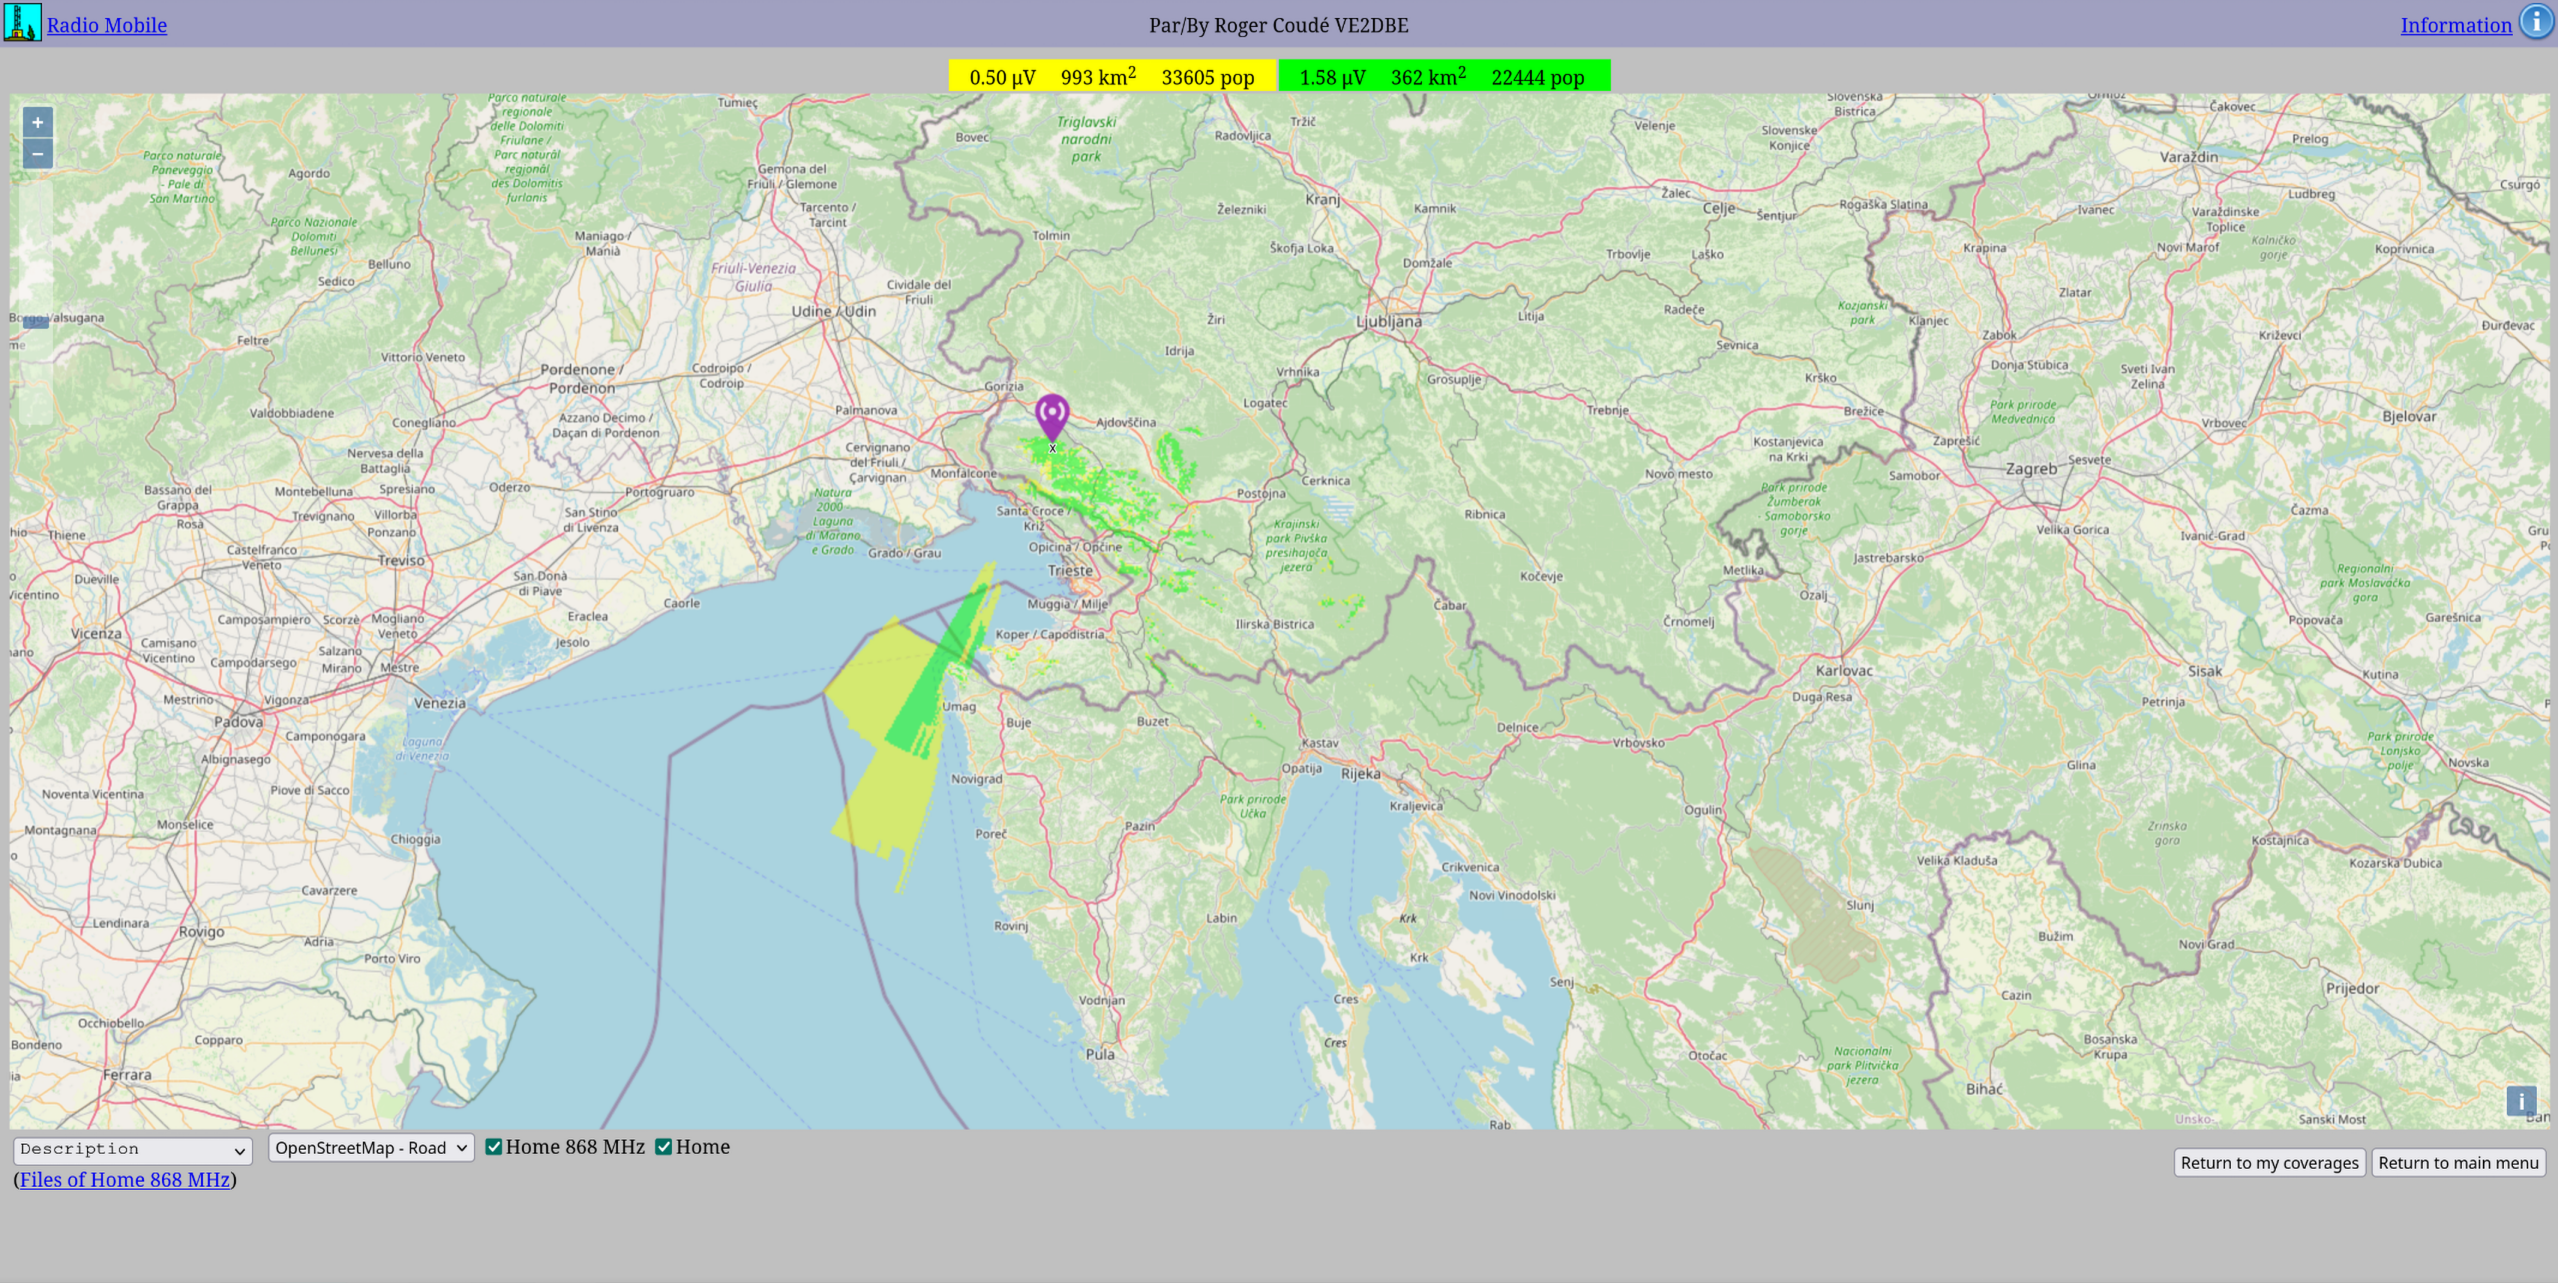
\includegraphics[width=1\textwidth]{fotografije/radio-mobile-online-celni-sistem.png}
\caption{Posnetek zaslona čelnega sistema sorodnega dela Radio Mobile Online}
\label{fig:radio-mobile-online}
\end{figure}

\subsection{SCADACore RF Line-of-Sight Calculator}
Orodje RF Line-of-Sight Calculator podjetja SCADACore~\cite{scadacoreRFLoS} je namenjeno preverjanju neposredne vidne linije med dvema točkama. Uporabniku omogoča hitro in enostavno oceno, ali med izbranima lokacijama obstaja neposredna vidna povezava. Kljub enostavni uporabi pa orodje ne podpira izračuna jakosti signala, analize Fresnelovih con ali vpliva frekvence, zato je uporabno predvsem kot informativno oziroma dopolnilno orodje.

\begin{figure}[htb]
\centering
\includegraphics[width=1\textwidth]{fotografije/scadacore-celni-sistem.png}
\caption{Posnetek zaslona čelnega sistema sorodnega dela SCADACore RF Line-of-Sight Calculator}
\label{fig:scadacore}
\end{figure}

\subsection{GRASS-RaPlaT}
RaPlaT (Radio Propagation and Terrain Analysis Tool)~\cite{raplatGrass,Ozimek2010GRASSRaPlaT} je odprtokodno orodje za modeliranje širjenja radijskega signala, ki temelji na geografskem informacijskem sistemu GRASS GIS. Omogoča uporabo različnih propagacijskih modelov nad prostorskimi podatki ter upošteva vpliv terena pri izračunu radijske pokritosti.

Glavna prednost orodja je njegova tesna integracija z GIS okoljem, ki omogoča natančno prostorsko analizo in uporabo različnih slojev geografskih podatkov. Njegova slabost pa je relativna zahtevnost uporabe, saj zahteva dobro poznavanje sistema GRASS GIS, dela z ukazno vrstico ter priprave prostorskih podatkov. Zaradi tega je RaPlaT primeren predvsem za raziskovalno in strokovno rabo, manj pa za hitro in intuitivno načrtovanje radijskih omrežij. Orodje prav tako ne ponuja neposredne analize vidne linije med poljubno izbranimi točkami.

\begin{figure}[htb]
\centering
\includegraphics[width=1\textwidth]{fotografije/ijs-raplat-celni-sistem.png}
\caption{Posnetek zaslona čelnega sistema sorodnega dela GRASS-RaPlaT}
\label{fig:raplat}
\end{figure}

Pregled sorodnih del pokaže, da obstoječa orodja praviloma ponujajo bodisi simulacijo pokritosti bodisi analizo vidne linije, redko pa oboje v integrirani in razširljivi obliki. Predstavljeno delo te omejitve naslavlja z združitvijo simulacij, vizualizacije in eksperimentalne evalvacije v enem odprtokodnem orodju.
\chapter{Uporabljene tehnologije in orodja}

Pri razvoju diplomske naloge so bila uporabljena sodobna orodja in tehnologije. Poleg tega so izbrane rešitve preverjene, odprtokodne ter široko uporabljane v industriji, kar zagotavlja stabilnost in dolgoročno vzdržnost sistema. V nadaljevanju so predstavljene ključne tehnologije in orodja, ki so bila uporabljena pri razvoju aplikacije, ter njihova vloga pri delovanju celotne rešitve.

\section{Vue.js}
Vue.js~\cite{vuejs} je odprtokodno ogrodje za gradnjo uporabniških vmesnikov, ki temelji na programskem jeziku JavaScript. Namenjen je gradnji enostranskih aplikacij z več manjšimi gradniki, ki jih je mogoče ponovno uporabiti na več različnih delih aplikacije. S tem se prihrani čas pri programiranju in zmanjša število vrstic kode.

Prva različica je ugledala luč sveta leta 2014. Zasnoval in ustvaril ga je Evan You kot izboljšavo ogrodja AngularJS~\cite{angularjs}, potem ko je z njim delal v podjetju Google.

\section{Tailwind CSS}
Tailwind CSS je sodobna knjižnica za oblikovanje, ki temelji na pristopu oblikovanja z razredi. Namesto pisanja lastnih slogov razvijalci uporabljajo vnaprej pripravljene razrede, kot so \texttt{ml-2}, \texttt{bg-orange-400} ali \texttt{block}, kar omogoča hitrejše prototipiranje in konsistenten dizajn. Ena od njegovih prednosti je tudi optimizacija za produkcijo, saj lahko odstrani neuporabljene razrede in s tem zmanjša velikost končne aplikacije.

\section{Python}
Python~\cite{python} je visokonivojski, interpretirani programski jezik, ki se odlikuje po enostavni in berljivi sintaksi. Njegove prednosti so obsežen standardni knjižnični nabor, aktivna skupnost ter široka podpora za različna področja – od spletnega razvoja in avtomatizacije do podatkovne znanosti in umetne inteligence. Python podpira več programerskih paradigem, vključno s postopkovnim, objektno usmerjenim in funkcijskim programiranjem. Zaradi enostavnega učenja in zmogljivosti je danes eden najbolj priljubljenih jezikov na svetu.

\section{SPLAT!}
SPLAT!~\cite{splatTool} (angl. \emph{Signal Propagation, Loss, And Terrain analysis tool}) je odprtokodno terminalsko orodje za analizo in simulacijo širjenja radijskega signala. Jedro orodja temelji na modelu Longley--Rice, znanem kot \emph{Irregular Terrain Model} (ITM), ter njegovi izboljšani različici \emph{Irregular Terrain with Obstructions Model} (ITWOM), ki omogočata napoved izgub poti in jakosti sprejetega signala ob upoštevanju razgibanega terena. SPLAT! pri izračunih uporablja digitalne modele višin, Fresnelove cone ter geometrijo vidne linije, kar omogoča realistično oceno pokritosti na frekvencah med 20~MHz in 20~GHz.

\section{Redis}
Redis~\cite{redis} je odprtokodna podatkovna baza v pomnilniku, ki uporablja model ključ-vrednost. Zasnovan je za hitro obdelavo podatkov z nizko zakasnitvijo in podpira različne podatkovne strukture, kot so seznami, množice, urejeni seznami in zgoščene tabele. Pogosto se uporablja kot predpomnilnik, sistem za sporočila ali podatkovna baza za časovno občutljive podatke.

\section{GeoServer}
GeoServer~\cite{geoserver} je odprtokodni strežnik, namenjen objavi in obdelavi prostorskih podatkov. Podpira standarde OGC (Open Geospatial Consortium), kot so WMS (Web Map Service), WFS (Web Feature Service) in WCS (Web Coverage Service). GeoServer omogoča dostop do prostorskih podatkov iz različnih virov (npr. shapefile, GeoTIFF, PostGIS) ter njihovo vizualizacijo in analizo. Zaradi svoje razširljivosti in združljivosti s številnimi GIS orodji je postal standardna rešitev za objavo prostorskih podatkov na spletu.

\section{Nginx}
Nginx~\cite{nginx} je odprtokodni spletni strežnik in posredniški strežnik (angl. \emph{reverse proxy}), ki se uporablja za strežbo statičnih vsebin, obdelavo zahtev HTTPS ter uravnoteženje obremenitve med strežniki. Zaradi svoje učinkovitosti, majhne porabe virov in zmožnosti hkratnega obravnavanja velikega števila povezav je postal ena najbolj priljubljenih rešitev za gostovanje spletnih aplikacij. Nginx podpira tudi modul za predpomnjenje in varnostne nastavitve, kar ga uvršča med ključne gradnike sodobne strežniške infrastrukture.

\section{Docker}
Docker~\cite{docker} je platforma za kontejnerizacijo, ki omogoča zagon aplikacij v izoliranih okoljih. Kontejnerji združujejo programsko opremo z vsemi njenimi odvisnostmi, kar omogoča enostaven prenos in reproducibilno izvajanje na različnih sistemih. Docker je postal standard v industriji, saj poenostavlja razvoj, testiranje in uvajanje aplikacij. Njegove prednosti so hitrost zagona, konsistenca med okolji in podpora za mikroservisno arhitekturo.

\chapter{Zahteve in arhitektura aplikacije}

Cilj aplikacije je ohraniti osnovno funkcionalnost izhodiščne rešitve aplikacije Meshtastic Site Planner~\cite{meshtasticSitePlanner}, tj. simulacijo radijske pokritosti, ter jo razširiti z dodatnimi funkcionalnostmi.

Razvita aplikacija mora uporabniku omogočati:
\begin{itemize}
    \item simulacijo radijske pokritosti oddajnika na izbranem geografskem območju na podlagi radijskega modela,
    \item analizo vidne linije (Line-of-Sight) med dvema izbranima točkama,
    \item iskanje optimalne lokacije oddajnika iz vnaprej določenega seznama potencialnih lokacij,
    \item iskanje optimalne lokacije oddajnika znotraj izbranega geografskega območja.
\end{itemize}

Funkcionalnosti so zasnovane tako, da uporabniku omogočajo primerjavo različnih scenarijev postavitve oddajnikov ter podporo pri odločanju o optimalni konfiguraciji omrežja.

\section{Arhitektura aplikacije}
Razvita aplikacija je zasnovana modularno in je sestavljena iz sedmih glavnih komponent:
\begin{itemize}
    \item čelnega sistema,
    \item zalednega sistema,
    \item simulacijskega orodja SPLAT!~\cite{splatTool},
    \item GIS-strežnika GeoServer~\cite{geoserver},
    \item podatkovnega strežnika Redis~\cite{redis},
    \item posredniškega strežnika Nginx~\cite{nginx},
    \item okolja Docker~\cite{docker}.
\end{itemize}

% Povezava do spodnjega diagrama https://app.diagrams.net/#G1StwCVnYQ4R7P79ZIJihRiKlY891dZTAp
\begin{figure}[htb]
\centering
\includegraphics[width=0.7\textwidth]{fotografije/arhitektura-aplikacije.png}
\caption{Arhitektura aplikacije za načrtovanje brezžičnih omrežij.}
\label{fig:arhitektura-aplikacije}
\end{figure}

\subsection{Čelni del}
Čelni del aplikacije predstavlja neposreden stik z uporabnikom in je razvit v ogrodju Vue.js~\cite{vuejs} z uporabo slogovne knjižnice Tailwind CSS~\cite{tailwindcss}, kar omogoča modularen razvoj in enostavno vzdrževanje uporabniškega vmesnika.

V začetni fazi razvoja je bila za oblikovanje uporabljena knjižnica Bootstrap~\cite{bootstrap}, ki pa je bila kasneje zamenjana z modernejšo in bolj prilagodljivo rešitvijo.

Osrednji element čelnega sistema je interaktivni zemljevid, zgrajen na knjižnici MapLibre GL~\cite{vueMapLibreGL, maplibre}, ki omogoča vizualizacijo rezultatov simulacij v obliki kartografskih slojev, markerjev in grafičnih prikazov jakosti signala. Prvotno uporabljena knjižnica Leaflet~\cite{leafletjs} se je izkazala za manj primerno pri delu z večjimi količinami prostorskih podatkov, zato je bila nadomeščena z zmogljivejšo alternativo.

Poleg zemljevida čelni sistem vključuje tudi obrazce za vnos parametrov simulacij ter pregledne prikaze rezultatov. Za zagotavljanje konsistentnosti podatkov se uporablja centralizirana shramba stanja, komunikacija z zalednim sistemom pa poteka prek REST API klicev.

\paragraph{Zaledni del}
Zaledni del je implementiran v programskem jeziku Python~\cite{python} z uporabo ogrodja FastAPI~\cite{fastapi}. Njegova glavna naloga je obdelava uporabniških zahtev, validacija vhodnih parametrov, priprava vhodnih datotek za simulacije, izvajanje izračunov ter posredovanje rezultatov čelnemu sistemu.

Pri zahtevnejših opravilih sistem deluje asinhrono: vsaki zahtevi dodeli enoličen identifikator, sproži simulacijo v ozadju in njen status ter vmesne rezultate začasno shrani v podatkovni strežnik Redis. Čelni sistem lahko nato periodično preverja stanje naloge in rezultate prevzame, ko so ti na voljo.

\paragraph{Baza podatkov}
Baza podatkov v arhitekturi deluje kot pomnilniški posrednik med čelnim in zalednim delom aplikacije. V njej se hranijo statusi opravil in končni rezultati simulacij. Aplikacija uporablja Redis~\cite{redis}, ki zaradi arhitekture ključ--vrednost in delovanja neposredno v pomnilniku omogoča zelo hitro shranjevanje in pridobivanje podatkov, kar prispeva k odzivnosti sistema.

\paragraph{Simulacijsko orodje}
Jedro simulacij predstavlja terminalsko orodje SPLAT!~\cite{splatTool}, ki na podlagi vhodnih parametrov, kot so moč oddajnika, višina antene, frekvenca delovanja, topografija terena in drugi fizikalni dejavniki, izračuna širjenje radijskega signala. Rezultati simulacij so lahko v obliki rastrskih podatkov, profilov signalne poti ali analiz vidne linije med posameznimi točkami. Orodje uporablja modele radijskega prenosa, ki upoštevajo vpliv zakritosti in Fresnelovih con, kar omogoča realistične simulacije in napoved pokritosti obravnavanega območja.

\paragraph{GIS strežnik}
Rezultati, ki jih ustvari simulacijsko jedro, se nadalje obdelajo in objavijo prek GIS-strežnika GeoServer~\cite{geoserver}. Izhodni podatki so pretvorjeni v format GeoTIFF in objavljeni kot spletne storitve, kot je na primer WMS. Čelni sistem te storitve nalaga dinamično in jih prikazuje kot sloje na interaktivnem zemljevidu, pri čemer se prenašajo le tisti deli podatkov, ki jih uporabnik dejansko potrebuje. Tak pristop omogoča učinkovito delo z velikimi količinami prostorskih podatkov ter zagotavlja skalabilno in zmogljivo vizualizacijo simulacij.

\paragraph{Posredniški strežnik}
Za usmerjanje prometa med posameznimi komponentami sistema skrbi spletni strežnik Nginx~\cite{nginx}, ki deluje kot povratni posrednik (angl. \emph{reverse proxy}). Poleg strežbe statičnih datotek čelnega sistema omogoča tudi obdelavo HTTPS povezav ter optimizacijo zmogljivosti z uravnavanjem obremenitve. S tem zagotavlja stabilno, varno in učinkovito komunikacijo med uporabniki in aplikacijo.

\paragraph{Platforma za kontejnerizacijo}
Celotna aplikacija je zapakirana z uporabo tehnologije Docker~\cite{docker}, ki omogoča zagon posameznih komponent v izoliranih in prenosljivih kontejnerjih. Vsaka storitev, kot so zaledni sistem, GeoServer in Redis, deluje v lastnem kontejnerju skupaj z vsemi potrebnimi odvisnostmi. Docker je bil uporabljen tako v fazi razvoja in testiranja kot tudi v produkcijskem okolju, kar zagotavlja konsistentnost delovanja, zmanjšuje možnost napak pri namestitvi ter omogoča enostavno posodabljanje in uvajanje novih verzij sistema.
\chapter{Implementacija}
Implementacija rešitve je razdeljena na dva glavna sklopa: zaledni del in čelni del aplikacije. Zaledni del skrbi za izvajanje simulacij radijskega širjenja, obdelavo višinskih podatkov, upravljanje opravil ter komunikacijo s simulacijskim orodjem SPLAT!. Čelni del predstavlja uporabniški vmesnik, ki omogoča vnos parametrov, upravljanje simulacij in vizualizacijo rezultatov na interaktivnem zemljevidu.

Jedro implementacije temelji na razširitvi obstoječe odprtokodne rešitve \texttt{Meshtastic Site Planner}~\cite{meshtasticSitePlanner}. Orodje omogoča simulacijo radijske pokritosti na podlagi orodja SPLAT! \cite{splatTool}, vendar ne podpira analize vidne linije ter iskanja optimalnih lokacij oddajnikov. Namesto razvoja celotnega sistema iz nič sem zato izvedel vejitev (angl.~\textit{fork}) projekta in ga nadgradil z dodatnimi funkcionalnostmi ter izboljšano arhitekturo.

Projekt \texttt{Meshtastic Site Planner} je licenciran pod licenco GPL~3~\cite{gpl3}, ki dovoljuje uporabo, spreminjanje in distribucijo programske opreme, ob pogoju, da so tudi izpeljana dela objavljena pod isto licenco. Tak licenčni model zagotavlja odprtost izvorne kode ter omogoča, da so vse nadaljnje izboljšave dostopne širši skupnosti. Izbrani pristop je omogočil hitrejši razvoj ter osredotočenost na razširitve sistema, kot so izboljšan prikaz rezultatov, pohitritev sistema ter dodajanje metod za iskanje optimalnih lokacij oddajnikov. Za prikaz rezultatov simulacij radijske pokritosti je v sistem vključen strežnik GeoServer, ki omogoča postopno nalaganje prostorskih podatkov prek vmesnika WMS ter s tem zmanjša obremenitev odjemalca.

\section{Zaledni del}
Zaledni del je implementiran v programskem jeziku Python~\cite{python}, pri čemer je za gradnjo spletnega vmesnika uporabljeno ogrodje FastAPI~\cite{fastapi}. Ogrodje omogoča enostavno vzpostavitev HTTP povezav ter olajša dodajanje in vzdrževanje funkcionalnosti REST API, ki so ključne za komunikacijo med čelnim in zalednim delom aplikacije.

Sistemu sem dodal dve novi API poti (angl.~\textit{routes}):
\begin{itemize}
    \item \textbf{POST /los} -- sproži simulacijo vidne linije (angl.~\textit{line-of-sight}) med dvema točkama,
    \item \textbf{DELETE /coverage/:task\_id} -- omogoča brisanje shranjenih rezultatov pokritosti.
\end{itemize}

Dve obstoječi poti sem preimenoval, da sledita poenotenemu poimenovanju:
\begin{itemize}
    \item \textbf{POST /predict} $\rightarrow$ \textbf{POST /coverage} -- sproži simulacijo radijske pokritosti glede na parametre oddajnika,
    \item \textbf{/status/:task\_id} $\rightarrow$ \textbf{GET /task} -- vrne stanje naloge in (ko so pripravljeni) dostop do rezultatov.
\end{itemize}

Poti \textbf{POST /los} in \textbf{POST /coverage} najprej validirata vhodne podatke glede na vnaprej definiran podatkovni model. Nato ustvarita novo nalogo, ji dodelita status \texttt{processing} ter začneta obdelavo zahtevka. Čelnemu delu aplikacije se vrne identifikator naloge, prek katerega je mogoče spremljati njeno stanje.

\subsection{Prenos in pretvorba digitalnih višinskih podatkov}
Višinski podatki so eden izmed ključnih gradnikov natančne simulacije širjenja radijskega signala, saj neposredno vplivajo na izračun vidne linije, zakritosti Fresnelovih con ter difrakcijskih izgub. Uporaba napačnih ali premalo natančnih digitalnih modelov višin lahko vodi do nerealnih napovedi pokritosti, bodisi v obliki precenjene jakosti signala bodisi v napačni identifikaciji ovir na poti signala.

Radijski modeli, kot je Longley--Rice (ITM), temeljijo na vzdolžnem profilu terena med oddajnikom in sprejemnikom, pri čemer lahko že razlike nekaj metrov v višini terena bistveno spremenijo izračunano zakritost prve Fresnelove cone in s tem končno napovedano izgubo poti. Raziskave kažejo, da imajo različne baze višin z različno prostorsko ločljivostjo in načinom zajema (npr.~SRTM, USGS NED, LIDAR) opazen vpliv na rezultate simulacij; grobejši modeli lahko spregledajo manjše terenske ovire ali pa zaradi šuma povzročijo umetno povečanje izgub signala~\cite{8077956}.

SPLAT! za delovanje potrebuje digitalne modele višin (DEM, angl.~\textit{Digital Elevation Model}), ki opisujejo višino terena in so praviloma na voljo v obliki datotek \texttt{.hgt}. Program je bil zasnovan za delo z višinskimi podatki misije \textit{Shuttle Radar Topography Mission (SRTM)}~\cite{srtm}, ki jih je NASA zbrala med 11-dnevno misijo februarja 2000. Rezultat misije je globalno usklajen digitalni model višin, ki pokriva približno 80~\% kopnega med 60$^\circ$ severne in 56$^\circ$ južne zemljepisne širine z ločljivostjo do 30~m.

Pred uporabo je treba surove višinske podatke pretvoriti v obliko, ki jo SPLAT! razume. Za to služita pripomočka \texttt{srtm2sdf} in \texttt{srtm2sdf-hd}, ki podatke iz formata \texttt{.hgt} pretvorita v format \texttt{.sdf} (\textit{Splat Data File}), ki omogoča hitrejše branje in obdelavo znotraj simulacijskega jedra.

Podatki misije SRTM so na voljo v dveh ločljivostnih različicah:
\begin{itemize}
  \item \textbf{SRTM3} -- ločljivost 3 ločne sekunde (približno 90~m med vzorci), skoraj globalna pokritost;
  \item \textbf{SRTM1} -- ločljivost 1 ločne sekunde (približno 30~m med vzorci), sprva omejena na ZDA, kasneje razširjena tudi na druge regije.
\end{itemize}

Orodje \texttt{srtm2sdf} omogoča pretvorbo podatkov SRTM3, medtem ko \texttt{srtm2sdf-hd} omogoča pretvorbo visoko ločljivostnih podatkov SRTM1 v izboljšan format \texttt{.sdf} z oznako \texttt{-hd}. Večja prostorska natančnost je posebej pomembna pri razgibanem terenu ali pri analizah na krajših razdaljah, kjer lahko že manjše razlike v višinskih podatkih vplivajo na rezultate simulacije.

V začetni fazi je zaledni del aplikacije samodejno izvajal pretvorbo iz \texttt{.hgt} v \texttt{.sdf}, kar je omogočalo izvajanje simulacij kjerkoli na svetu, vendar je postopek podaljšal čas obdelave in poslabšal uporabniško izkušnjo. Za optimizacijo sem uporabil vir \texttt{viewfinderpanoramas.org}~\cite{viewfinder}, ki ponuja že pripravljene in preverjene višinske ploščice v ustreznem formatu. Ploščice za območje Evrope sem prenesel in shranil na lasten strežnik, od koder jih aplikacija po potrebi samodejno pridobi in uporabi pri izvajanju simulacij. S tem se zmanjša zakasnitev ob začetku izračuna ter izboljša odzivnost sistema pri ponavljajočih se simulacijah.

\subsection{Določanje potrebnih višinskih ploščic za simulacije}

Za izvajanje simulacij SPLAT! potrebuje ustrezen nabor višinskih ploščic (\texttt{.sdf}), ki pokrivajo območje analize. V izvorni aplikaciji je bil postopek določanja potrebnih ploščic že implementiran za simulacijo radijske pokritosti, pri čemer se upošteva celoten okoliš oddajnika znotraj izbranega polmera.

Na podlagi izbranega polmera in geografske lokacije oddajnika se najprej določi omejitveni pravokotnik (angl.~\textit{bounding box}), ki zajema celotno območje simulacije. Nato se iz tega območja izpelje seznam višinskih ploščic, ki jih je treba prenesti in vključiti v izračun. Tak pristop omogoča, da se obdelujejo le nujno potrebni podatki, s čimer se zmanjša količina prenesenih višin\-skih podatkov in pospeši priprava simulacije.

Ker izvorna aplikacija ni podpirala analize vidne linije (LOS), sem obstoječi mehanizem razširil tudi za ta primer. Pri simulaciji vidne linije je območje interesa omejeno zgolj na zveznico med oddajnikom in sprejemnikom, zato je mogoče nabor potrebnih ploščic dodatno zožiti. Namesto celotnega območja okoli oddajnika se določijo le tiste ploščice, ki jih prečka povezovalna linija med obema točkama.

S tem je bil obstoječi sistem za določanje višinskih ploščic ponovno uporabljen in prilagojen tudi za simulacijo vidne linije, kar omogoča učinkovitejšo rabo podatkov ter krajši čas priprave izračuna, zlasti pri točkovnih analizah na večjih razdaljah.


\subsection{Lokacija oddajnika / sprejemnika}
SPLAT! za določitev geografskih lokacij oddajnika in sprejemnika uporablja \textbf{.qth} datoteke (angl.~\textit{QTH files}), 
ki vsebujejo osnovne podatke o analiziranih točkah. Datoteka je navadna besedilna datoteka v obliki ASCII in ima štiri vrstice:

\begin{enumerate}
  \item ime lokacije (npr.~oznaka oddajnika ali sprejemnika),
  \item geografska širina (v decimalnih stopinjah, pozitivna za severno poloblo, negativna za južno),
  \item geografska dolžina (v stopinjah zahodno od Greenwicha od 0~do~360 ali vzhodno od~0~do~--360),
  \item višina antene nad tlemi (\textit{AGL – Above Ground Level}) v metrih ali čevljih.
\end{enumerate}

Primer datoteke:
\begin{verbatim}
WNJT-DT
40.2828
74.6864
990.00
\end{verbatim}

V zadnji vrstici se privzeto predpostavi, da je višina podana v čevljih, razen če je za številčno vrednostjo navedena enota \texttt{m} ali beseda \texttt{meters}.  
Latitude in longitude se lahko zapišeta v decimalnem formatu (npr.~\texttt{46.0500}) ali v formatu stopinje–minute–sekunde (npr.~\texttt{46 3 0.0}).  
Vsak analiziran oddajnik in sprejemnik mora imeti svojo lastno \texttt{.qth} datoteko, ki jo program naloži ob izvajanju simulacije.

SPLAT! pričakuje nekoliko drugačno predstavitev dolžine kot standard EPSG:4326 (WGS84), ki jo uporablja večina sodobnih GIS sistemov.  
V EPSG:4326 so pozitivne vrednosti dolžin vzhodno od Greenwicha, negativne pa zahodno.  
SPLAT! pa zahteva pozitivne vrednosti za zahodno poloblo (0~do~360°~W) in negativne za vzhodno (0~do~--360°~E).  
Da zagotovimo pravilno interpretacijo, se v aplikaciji uporablja naslednja pretvorba:

\[
\lambda_{\mathrm{SPLAT}} =
\begin{cases}
|\lambda|, & \lambda < 0 \quad (\text{zahodne dolžine})\\[4pt]
360 - \lambda, & \lambda \ge 0 \quad (\text{vzhodne dolžine})
\end{cases}
\]

ali v implementacijski obliki:

\begin{verbatim}
longitude_splat = abs(longitude) if longitude < 0 else 360 - longitude
\end{verbatim}

S tem se zagotovita pravilna orientacija in skladnost z vhodnim formatom, ki ga pričakuje orodje SPLAT!.

\subsection{Parametri radijskega modela}
Poleg lokacijskih datotek \texttt{.qth} SPLAT! za vsako simulacijo uporablja tudi \textbf{.lrp} datoteko 
(angl.~\textit{Irregular Terrain Model Parameter file}), ki določa fizikalne in statistične parametre modela 
Longley–Rice (ITM – \textit{Irregular Terrain Model}).  

Datoteka \texttt{.lrp} vsebuje osem (po izbiri devet) vrstic, pri čemer vsaka določa en parameter modela:

\begin{itemize}
  \item \textbf{Dielektrična konstanta in prevodnost tal} določata elektromagnetne lastnosti podlage; 
  tipične vrednosti so 15 in 0.005~S/m za povprečna tla.  
  \item \textbf{Atmosferska refrakcijska konstanta} (privzeto 301~N) opisuje ukrivljanje radijskih valov zaradi sprememb lomnega količnika v atmosferi.
  \item \textbf{Frekvenca} določa območje uporabe modela (20~MHz–20~GHz).  
  \item \textbf{Radijska klima} (1–7) opisuje povprečne podnebne pogoje: 
  npr.~1~=~ekvatorialna, 5~=~celinsko zmerna (privzeto), 7~=~maritimna nad morjem.  
  \item \textbf{Polarizacija} označuje orientacijo elektromagnetnega polja (0~=~horizontalna, 1~=~vertikalna).  
  \item \textbf{Delež lokacij} in \textbf{delež časa} opredeljujeta statistični kriterij F($p$,~$q$), npr.~F(50,90), 
  kar pomeni, da bo največja izguba poti nastopila v 50~\% situacij 90~\% časa.  
  Ta kriterij je standardno uporabljen pri modelih Longley–Rice.
\end{itemize}

Če je zadnji parameter (ERP) izpuščen, SPLAT! izračuna zgolj \textit{path loss} (izgubo poti).  
Če je vključen, pa izvede tudi izračun jakosti električnega polja in kontur pokritosti (\textit{field strength}).

\paragraph{Izračun efektivne sevalne moči (ERP).}
Vrednost ERP izračunamo na podlagi nastavitev oddajnika po formuli:

\[
\text{ERP}_{\mathrm{dBm}} = P_\mathrm{TX}(\mathrm{dBm}) + \bigl(G_\mathrm{ant}(\mathrm{dBi}) - 2.15\bigr) - L_\mathrm{izgube}(\mathrm{dB})
\]

pri čemer:
\begin{itemize}
  \item $P_\mathrm{TX}$ predstavlja oddajno moč oddajnika,
  \item $G_\mathrm{ant}$ je ojačanje antene glede na izotropno anteno (v dBi),
  \item $L_\mathrm{izgube}$ so sistemske izgube (kabli, konektorji, dušilci).
\end{itemize}

Če želimo ERP izraziti v vatih, uporabimo:
\[
\text{ERP}_{\mathrm{W}} = 10^{\frac{(\text{ERP}_{\mathrm{dBm}} - 30)}{10}}.
\]

Za razliko od originala moja verzija aplikacije pričakuje pridobitek antene v dBi formatu, saj tega proizvajalci večkrat definirajo v specifikacijah antene. Zato v formuli najdemo \[
\mathrm{dBm} = \mathrm{dBi} - 2.15
\]

Konstanta 2.15~dB predstavlja razliko med izotropno referenčno anteno in dipolno referenčno anteno. 
Pridobitek antene je v praksi pogosto podan v enotah dBi, kjer je referenca idealna izotropna antena, ki enakomerno seva v vse smeri. 
Model Longley--Rice in s tem orodje SPLAT! pa uporabljata efektivno sevalno moč (ERP), ki je definirana glede na idealni polvalovni dipol (dBd). 
Razmerje med obema referencama je 2.15~dB, zato je za pretvorbo iz dBi v dBd potrebno odšteti 2.15~dB.

Tako izračunana ERP vrednost se zapiše v zadnjo vrstico \texttt{.lrp} datoteke.

\subsection{Barvna lestvica za prikaz moči signala}
Pri simulacijah radijske pokritosti SPLAT! uporablja datoteko \textbf{.dcf} (angl.~\textit{dBm Color Definition File}), 
ki določa barvno lestvico za prikaz nivojev sprejete moči v enotah dBm.  
Ta datoteka ni potrebna pri analizi vidne linije (LOS), saj se tam rezultati ne prikazujejo v obliki kontur, 
temveč le kot enodimenzionalen profil terena.  
Uporablja se torej izključno pri območnih simulacijah.

\paragraph{Struktura datoteke.}
Vsaka vrstica v datoteki \texttt{.dcf} določa razpon jakosti signala in pripadajočo barvo v RGB formatu (0–255)

SPLAT! podpira do 32 različnih barvnih nivojev, ki jih interpolira med največjo in najmanjšo vrednostjo.  
Barvna lestvica omogoča hitro vizualno interpretacijo jakosti signala na karti, kjer rdeči toni označujejo 
najmočnejše vrednosti, modri in vijolični pa območja šibkega signala.

\paragraph{Avtomatsko generiranje datoteke.}
Za dinamično generiranje datoteke \texttt{.dcf} je v zalednem delu implementiran postopek, ki samodejno izdela vsebino na podlagi izbrane barvne karte (angl.~\textit{colormap}) iz knjižnice \texttt{Matplotlib}. Aplikacija generira 32 barvnih korakov med podanima mejama \texttt{min\_dbm} in \texttt{max\_dbm} ter jih zapiše v besedilni obliki.

Tako ustvarjena vsebina se pretvori v bajtni zapis in posreduje programu SPLAT! kot vhodna datoteka. Postopek omogoča, da ima uporabnik možnost izbire različnih barvnih shem (npr.~\texttt{viridis}, \texttt{plasma}, \texttt{turbo}) ter da sistem prilagodi vizualni prikaz pokritosti brez ročnega urejanja datotek.

\paragraph{Uporaba.}
Datoteka \texttt{.dcf} se uporabi le pri simulacijah pokritosti, 
kjer je v \texttt{.lrp} datoteki ali prek parametra \texttt{-erp} določena efektivna sevalna moč oddajnika (ERP).  
V tem primeru SPLAT! namesto kontur izgub (\texttt{.lcf}) ali polj jakosti (\texttt{.scf}) 
uporabi definicije barv iz \texttt{.dcf} za prikaz sprejete moči v dBm.  
Pri analizi vidne linije (\texttt{-c}) se ta datoteka ne uporablja, saj se tam generirajo le geometrijski rezultati brez barvnih kontur.


\subsection{Izvedba simulacije}

Simulacija se izvede s klicem zunanjega programa SPLAT! oziroma SPLAT-HD, odvisno od izbrane ločljivosti terenskih podatkov. Oba programa imata enak nabor ukaznih parametrov (\textit{flagov}), ki določajo vhodne datoteke, fizične parametre modela in izhodne formate. Zaledni sistem zgradi ukazno vrstico glede na vrsto zahteve – bodisi analizo vidne linije (LOS) bodisi izračun pokritosti (Coverage Prediction) – in jo zažene v ločenem procesu znotraj začasne mape.

Najpogosteje uporabljeni parametri so:
\begin{itemize}
  \item \texttt{-t} – pot do datoteke z oddajnikom (\texttt{tx.qth});
  \item \texttt{-r} – pot do datoteke s sprejemnikom (\texttt{rx.qth});
  \item \texttt{-L} – višina sprejemne antene (v metrih);
  \item \texttt{-R} – polmer območja izračuna (v kilometrih);
  \item \texttt{-f} – delovna frekvenca v MHz za izračun Fresnelovih con;
  \item \texttt{-gc} – višina talne oviranosti (vegetacija, objekti);
  \item \texttt{-db} in \texttt{-dbm} – prag in način prikaza jakosti signala;
  \item \texttt{-kml} – izvoz v format, združljiv z orodjem Google Earth;
  \item \texttt{-gpsav} – ohrani začasne \texttt{gnuplot} datoteke;
  \item \texttt{-metric} – uporaba metričnega sistema enot;
  \item \texttt{-olditm} – uporaba standardnega modela ITM (Longley–Rice) namesto model ITWOM;
\end{itemize}

\subsubsection*{Analiza vidne linije (LOS)}
Pri analizi vidne linije se oceni, ali med oddajnikom in sprejemnikom obstaja neposredna vidna povezava. Program se zažene s sledečim nizom parametrov:
\begin{verbatim}
splat_command = [
    (self.splat_hd_binary if request.high_resolution else self.splat_binary),
    "-t", "tx.qth",
    "-r", "rx.qth",
    "-H", "normalized_terrain_height_graph.png",
    "-d", self.tile_cache,
    "-f", f"{request.frequency_mhz}M",
    "-gc", str(request.clutter_height),
    "-gpsav",
    "-metric",
    "-olditm",
]
\end{verbatim}

Po zagonu se v začasni mapi ustvarijo različne izhodne datoteke, ki opisujejo profil poti med točkama: višinski profil (\texttt{profile.gp}), krivino Zemlje (\texttt{curvature.gp}), prvo Fresnelovo cono (\texttt{fresnel.gp}), referenčno višinsko linijo (\texttt{reference.gp}) in tekstovno poročilo (\texttt{tx-to-rx.txt}). Te datoteke se nato odčitajo in združijo v strukturiran JSON odgovor, ki vključuje:
\begin{itemize}
  \item numerične podatke o profilu terena in Fresnelovih conah,
  \item informacijo, ali je pot optično prosta ali ovirana,
  \item izračunano izgubo poti po modelu ITM in jakost sprejetega signala (v~dBm),
  \item seznam geografskih koordinat ovir na poti.
\end{itemize}

Tako dobljeni rezultat se vrne odjemalcu, kjer se podatki uporabijo za vizualizacijo profila poti in označevanje ovir. Sistem vmes ohrani tudi vse začasne datoteke, kar omogoča njihovo kasnejšo analizo ali ponovno uporabo brez ponovnega izračuna.

\subsubsection*{Izračun pokritosti (Coverage Prediction)}
Pri simulaciji pokritosti se izvede prostorski izračun jakosti signala na območju okoli oddajnika v danem polmeru. Za ta namen se uporabi model Longley–Rice (ITM), ki izračuna pričakovano moč signala za vsako točko znotraj območja. Program se zažene z naslednjimi parametri:
\begin{verbatim}
splat_command = [
    (self.splat_hd_binary if request.high_resolution else self.splat_binary),
    "-t", "tx.qth",
    "-L", str(request.rx_height),
    "-o", "output.ppm",
    "-d", self.tile_cache,
    "-R", str(request.radius),
    "-f", f"{request.frequency_mhz}M",
    "-gc", str(request.clutter_height),
    "-db", str(request.min_dbm),
    "-dbm",
    "-sc",
    "-ngs",
    "-N",
    "-kml",
    "-gpsav",
    "-metric",
    "-olditm",
]
\end{verbatim}

Rezultat simulacije vključuje več datotek:
\begin{itemize}
  \item \texttt{output.ppm} – barvni zemljevid jakosti signala,
  \item \texttt{output-ck.ppm} – barvna legenda (color key),
  \item \texttt{output.kml} – prostorska referenca in obseg simuliranega območja.
\end{itemize}

Ohranil sem pretvorbo iz \texttt{.ppm} v \texttt{.tif}. Datoteka \texttt{.ppm} se prebere in pretvori v enokanalno matriko sivinskih vrednosti, medtem ko datoteka \texttt{.kml} vsebuje meje območja (koordinate sever, jug, vzhod, zahod), ki omogočajo georeferenciranje. Na podlagi teh podatkov se z uporabo knjižnice \texttt{rasterio} in funkcije \texttt{from\_bounds()} izdela GeoTIFF slika, pri čemer se ustvari barvna lestvica iz izbranega \texttt{Matplotlib} kolormap-a in dBm razpona. Nastavi se tudi vrednost \texttt{nodata} za prosojna območja in priloži GDAL-združljiv barvni zemljevid.

Dodal pa sem, da se pripravljen GeoTIFF nato shrani v pomnilnik in preko funkcije \texttt{store\_tiff\_in\_geoserver()} posreduje strežniku GeoServer, kjer se zapiše kot nov \textit{coverage store} in postane dostopen prek standardnega WMS vmesnika. Istočasno se v Redis zapiše status opravila ter podatkovni ključ z rezultatom (vključno z legendo, kodirano v~\texttt{Base64}).


\section{Čelni sistem}

Čelni sistem aplikacije je zasnovan kot osrednja točka interakcije med uporabnikom in simulacijskim jedrom. Njegova glavna naloga je omogočiti enostaven vnos parametrov, pregledno upravljanje simulacij ter intuitivno vizualizacijo rezultatov na interaktivnem zemljevidu.

Arhitektura čelnega sistema je v osnovi ostala podobna izvorni rešitvi \textit{Meshtastic Site Planner} \cite{meshtasticSitePlanner}, vendar je bila nadgrajena z modernejšimi tehnologijami in izboljšanimi komponentami. Za oblikovanje uporabniškega vmesnika sem namesto ogrodja Bootstrap \cite{bootstrap} uporabil ogrodje Tailwind CSS \cite{tailwindcss}, ki omogoča bolj fleksibilno in konsistentno oblikovanje ter hitrejši razvoj brez potrebe po pisanju obsežnih lastnih slogovnih datotek.

Pomembna sprememba je bila tudi zamenjava knjižnice Leaflet \cite{leafletjs} z Vue MapLibre GL \cite{vueMapLibreGL}. Nova rešitev omogoča boljšo zmogljivost pri prikazu večjih količin prostorskih podatkov, boljšo podporo za delo z vektorskimi sloji ter večjo prilagodljivost pri izrisu  elementov.


\subsection{Simulacija vidne linije}
Pomembna funkcionalnost, ki sem jo dodal v aplikacijo, je simulacija vidne linije (angl.~\textit{Line-of-Sight}, LOS) med dvema izbranima točkama.

Uporabnik lahko v čelnem sistemu izbere točki z neposrednim klikom na zemljevid ali z vnosom geografskih koordinat. Ob potrditvi aplikacija prek API-klica posreduje podatke zalednemu sistemu, ki jih obdela in pošlje programu SPLAT! za izračun vidne linije.

Rezultat analize vključuje informacijo, ali med točkama obstaja neposredna vidljivost, ter profil terena na poti signala. V profilu so označene morebitne ovire, ki lahko vplivajo na kakovost povezave, vključno z zakritjem Fresnelovih con.

V čelnem sistemu se rezultat prikaže v obliki grafa profila poti, ki uporabniku omogoča natančen vpogled v razmere med oddajnikom in sprejemnikom. Graf vključuje več elementov:
\begin{itemize}
  \item \textbf{Direktno linijo} med antenama, ki ponazarja teoretično neovirano pot signala;
  \item \textbf{Krivino Zemlje} (angl.~\textit{Earth curvature}), ki prikazuje vpliv zemeljske ukrivljenosti na višinsko razliko med točkama;
  \item \textbf{Fresnelovo cono} (angl.~\textit{Fresnel zone}), ki ponazarja območje, znotraj katerega morata biti prepreke minimalne za nemoteno širjenje signala;
  \item \textbf{Fresnelovo cono 60\,\%}, ki predstavlja prag, do katerega se tolerira delno zakritje brez večjih izgub;
  \item \textbf{Pričakovano jakost sprejetega signala (RSSI)} v~dBm, ki upošteva moč oddajnika, ojačitev anten in izgube na poti;
  \item \textbf{Izgubo poti (Path loss)}, izraženo v~dB, ki predstavlja razliko med močjo oddanega in sprejetega signala.
\end{itemize}

Vsi podatki se prikažejo interaktivno: uporabnik lahko premika kazalec po profilu, da odčita višino terena in druge izračunane vrednosti za posamezno razdaljo. Barvna legenda jasno razlikuje posamezne plasti grafa (teren, direktno linijo, Fresnelove cone in krivino Zemlje), kar omogoča hitro vizualno oceno morebitnih ovir na poti.

Graf je interaktiven in povezan z zemljevidom. Ko se uporabnik z miško premika po profilu poti, se na zemljevidu istočasno prikaže ustrezna točka na terenu. Na ta način lahko uporabnik hitro prepozna natančno lokacijo posamezne ovire ali območja, kjer signal izgubi vidno linijo.  
Sinhronizacija med grafom in zemljevidom omogoča intuitivno analizo – uporabnik ne vidi le numeričnih vrednosti, temveč tudi prostorski kontekst, kar izboljša razumevanje rezultatov in načrtovanje postavitve anten.

\begin{figure}[htb]
\begin{center}
\includegraphics[width=0.8\textwidth]{fotografije/simulacija-vidnega-polja-graf.png}
\end{center}
\caption{Prikaz funkcionalnosti simulacije vidnega polja v čelnem sistemu aplikacije.}
\label{simulacija-vidnega-polja-graf}
\end{figure}

Tak prikaz uporabniku omogoča takojšnje razumevanje, kako teren vpliva na vidljivost in jakost signala, ter predstavlja pomembno orodje pri načrtovanju točkovnih povezav.

\begin{figure}[htb]
\begin{center}
\includegraphics[width=1\textwidth]{fotografije/simulacija-vidnega-polja-celni-sistem.png}
\end{center}
\caption{Prikaz funkcionalnosti simulacije vidnega polja v čelnem sistemu aplikacije.}
\label{simulacija-vidnega-polja-celni-sistem}
\end{figure}

\subsection{Simulacija radijske pokritosti}
Funkcionalnost simulacije radijske pokritosti (angl.~\textit{Coverage Prediction}) je bila v aplikaciji že prisotna, vendar sem jo nadgradil tako, da zdaj temelji na izrisu pokritosti v obliki GeoTIFF datoteke. Po izvedeni simulaciji se GeoTIFF zapiše na strežnik GeoServer, ki služi kot namenski sistem za prostorsko vizualizacijo in shranjevanje geografskih podatkov.

GeoServer omogoča dostop do prostorskih slojev prek standardiziranega protokola \textit{Web Map Service} (WMS). Namesto da bi se celoten rezultat prenesel hkrati, se uporabniku prenašajo le tiste ploščice (\textit{tiles}), ki jih trenutno vidi na zemljevidu. Tak pristop bistveno zmanjša količino prenesenih podatkov in omogoča sprotno nalaganje slojev glede na pogled uporabnika.

Vsaka ploščica prikazuje del območja pokritosti, pri čemer barvna lestvica označuje jakost signala v dBm. V ozadju GeoServer samodejno razdeli GeoTIFF v mrežo ploščic in jih posreduje odjemalcu glede na izbrano povečavo (angl.~\textit{zoom level}). Na strani čelnega sistema se ploščice nalagajo dinamično kot prekrivni sloj nad osnovnim zemljevidom, uporabnik pa lahko s spremembo povečave ali premikom zemljevida hitro razišče različne dele območja.

Kljub optimiziranemu prenosu ploščic je postopek še vedno časovno zahteven, zlasti pri uporabi visoko\-ločljivostnih podatkov (\texttt{splat-hd}). Ti podatki uporabljajo teren z ločljivostjo 1~ločne sekunde (približno 30~m), kar pomeni večjo količino podatkov za obdelavo in večje GeoTIFF datoteke. Pri takšnih izračunih se čas generiranja in nalaganja ploščic občutno poveča, saj se mora za vsako simulacijo prenesti in obdelati bistveno več višinskih ploščic ter ustvariti večji raster za izris pokritosti.  

Ko uporabnik v čelnem sistemu odstrani posamezno plast pokritosti, se sproži tudi ustrezen API-klic v zaledni sistem, ki izvede brisanje sloja iz GeoServerja. S tem se izogne nepotrebnemu kopičenju podatkov in ohranja strežnik čist, kar prispeva k boljšemu nadzoru nad porabo prostora ter stabilnosti sistema.

Tak pristop omogoča učinkovito in prilagodljivo delo z velikimi prostorskimi podatki, saj uporabnik prejme le tisti del informacij, ki jih v danem trenutku potrebuje, sistem pa hkrati samodejno skrbi za vzdrževanje in čiščenje podatkovne baze na strežniku.



\begin{figure}[htb]
\begin{center}
\includegraphics[width=1\textwidth]{fotografije/simulacija-radijske-pokritosti-celni-sistem.png}
\end{center}
\caption{Prikaz funkcionalnosti simulacije radijske pokritosti v čelnem sistemu aplikacije.}
\label{pic1}
\end{figure}

\subsection{Iskanje optimalnega centralnega oddajnika iz seznama oddajnikov}
Druga funkcionalnost aplikacije, ki sem jo implementiral, je \texttt{Center Node Simulator}, ki omogoča iskanje optimalne lokacije oddajnika glede na več izbranih sprejemnikov. Cilj te funkcionalnosti je določiti takšno lokacijo oddajnika iz nabora vnaprej znanih lokacij, ki zagotavlja najboljšo možno pokritost do vseh izbranih sprejemnikov.

Uporabnik na zemljevidu izbere več lokacij sprejemnikov ali jih vnese z uporabo geografskih koordinat. Nato določi nabor možnih lokacij oddajnikov, ki jih bo aplikacija analizirala. Za vsako izmed teh lokacij se izvede simulacija širjenja radijskega signala, na podlagi katere se izračuna pričakovana jakost signala za vse izbrane sprejemnike.

Rezultati simulacij so prikazani v pregledni tabeli, ki vsebuje kombinacije oddajnikov in sprejemnikov ter pripadajoče pričakovane vrednosti jakosti signala (RSSI) za posamezno povezavo. Uporabnik lahko podatke razvršča po posameznih stolpcih ali pa v spustnem seznamu izbere agregacijsko merilo, kot so \texttt{Average}, \texttt{Min} ali \texttt{Max}. Možnost \texttt{Average} razvrsti oddajnike glede na najvišjo povprečno vrednost RSSI, možnost \texttt{Min} glede na najnižjo izmerjeno vrednost RSSI, možnost \texttt{Max} pa glede na najvišjo vrednost RSSI. Na podlagi teh kriterijev lahko uporabnik izbere lokacijo oddajnika, ki predstavlja optimalen kompromis med pokritostjo in kakovostjo sprejema.


\begin{figure}[htb]
\begin{center}
\includegraphics[width=1\textwidth]{fotografije/simulacija-optimalne-centralne-tocke-celni-sistem.png}
\end{center}
\caption{Prikaz delovanja funkcionalnosti \texttt{Center Node Simulator} z izbranimi lokacijami sprejemnikov in izračunano optimalno lokacijo oddajnika.}
\label{pic:center-node}
\end{figure}

\subsection{Iskanje optimalnega centralnega oddajnika znotraj območja}
Tretja funkcionalnost aplikacije, ki sem jo implementiral, je \texttt{Area Center Node Simulator}, ki omogoča iskanje optimalne lokacije oddajnika znotraj uporabniško definiranega geografskega območja. Funkcionalnost je namenjena uporabnikom, ki ne želijo vnaprej določiti vseh možnih lokacij oddajnikov, temveč želijo, da aplikacija sama identificira primerne kandidatske lokacije.

Uporabnik na zemljevidu določi potencialne lokacije sprejemnikov in s poligonom označi območje iskanja lokacije oddajnika. Aplikacija nato s pomočjo podatkov OpenStreetMap~\cite{openstreetmap}, pridobljenih prek vmesnika Overpass API~\cite{overpass_api}, izlušči seznam vrhov znotraj izbranega območja. V podatkovnem modelu OpenStreetMap so vrhovi označeni z oznako \texttt{natural=peak}. Te lokacije se uporabijo kot kandidatske točke za postavitev oddajnika.

Za vsako izmed pridobljenih lokacij se izvede simulacija širjenja radijskega signala, na podlagi katere se izračuna pričakovana jakost signala za vse izbrane sprejemnike. Rezultati so prikazani v pregledni tabeli, ki vsebuje kombinacije oddajnikov in sprejemnikov ter pripadajoče vrednosti jakosti signala.

Na koncu uporabnik na podlagi enakih kriterijev kot pri funkcionalnosti iskanja optimalnega oddajnika iz vnaprej določenega seznama izbere lokacijo, ki predstavlja optimalno razmerje med pokritostjo in kakovostjo sprejema. Ključna razlika med obema funkcionalnostma je v načinu določanja kandidatskih lokacij oddajnika, medtem ko je postopek evalvacije in predstavitve rezultatov enak.


\begin{figure}[htb]
\begin{center}
\includegraphics[width=1\textwidth]{fotografije/simulacija-optimalne-centralne-tocke-obmocje-celni-sistem.png}
\end{center}
\caption{Prikaz delovanja funkcionalnosti \texttt{Area Center Node Simulator} z izbranimi sprejemniki, označenim območjem iskanja in izračunano optimalno lokacijo oddajnika.}
\label{pic:center-node-area}
\end{figure}
\chapter{Eksperimentalna evalvacija}
Celostna evalvacija implementirane rešitve bi lahko zajemala več različnih vidikov, med drugim preverjanje izpolnjevanja vseh funkcijskih zahtev, določenih v fazi načrtovanja, ocenjevanje uporabniškega vmesnika in uporabniške izkušnje s pomočjo uporabniške študije ter analizo učinkovitosti izvedbe aplikacije, kot so odzivnost sistema, čas izvajanja simulacij in poraba sistemskih virov.

Ker takšna celovita evalvacija presega obseg diplomskega dela, se to delo osredotoča na eksperimentalno evalvacijo natančnosti razvite aplikacije. Natančnost simulacij predstavlja temeljno lastnost orodja za radijsko

Z eksperimentalno evalvacijo je bila preverjena natančnost razvite aplikacije ter temeljnega propagacijskega sistema SPLAT!, ki se uporablja za simulacijo radijskega širjenja. Evalvacija je bila izvedena na podlagi dejanskih terenskih meritev v realnem okolju, pri čemer je bila uporabljena obstoječa infrastruktura omrežja Meshtastic. Takšen pristop je omogočil izvajanje ponovljivih in nadzorovanih meritev v realnih pogojih delovanja sistema.

\paragraph{Meshtastic}
Meshtastic~\cite{meshtasticFirmware} je odprtokodna platforma za vzpostavljanje nizkoenergijskih brezžičnih omrežij na osnovi tehnologije LoRa, ki omogoča decentralizirano komunikacijo med večjim številom vozlišč v mrežnem tipu omrežja (angl. \emph{mesh network}). Vsako vozlišče lahko deluje kot oddajnik, sprejemnik in posrednik sporočil, kar omogoča razširjanje dosega omrežja brez potrebe po centralni infrastrukturi. Sistem omogoča dostop večjemu številu odjemalcev ter izmenjavo telemetrijskih in lokacijskih podatkov, hkrati pa
podpira integracijo z zunanjimi sistemi, na primer prek protokola MQTT, kar omogoča centralizirano zbiranje in analizo podatkov iz omrežja.

\section{Strojna in programska oprema}
Meritve so bile izvedene z uporabo odprtokodne programske opreme Meshtastic~\cite{meshtasticFirmware}, ki omogoča pošiljanje lokacijskih paketov ter njihovo posredovanje prek protokola MQTT. Sprejeti podatki so se samodejno shranjevali v podatkovno bazo skupaj s pripadajočimi metapodatki, kot so čas prejema, identifikacija oddajnika in sprejemnika ter izmerjena jakost signala (RSSI).

Uporabljena strojna oprema temelji na cenovno dostopnih mikrokontrolerjih ESP32 in nRF52 z vgrajeno podporo za komunikacijo LoRa. V eksperimentalnem okolju so bila uporabljena naslednja vozlišča:

\begin{itemize}
    \item Statično vozlišče \texttt{!7369fb6a}, ki temelji na platformi \href{https://store.rakwireless.com/products/wisblock-meshtastic-starter-kit}{\texttt{RAK Wireless RAK4631}}, opremljeni z anteno \href{https://www.alfa.com.tw/products/aoa-868-5acm?variant=36473962922056}{\texttt{Alfa 868~MHz 5~dBi}}.
    \item Statično vozlišče \texttt{!75f19024}, ki temelji na platformi \href{https://lilygo.cc/products/t3s3-v1-0}{\texttt{LilyGo T3 S3}}, opremljeni z anteno \href{https://mikrotik.com/product/868_omni_antenna}{\texttt{MikroTik 868~MHz 6.5~dBi}}.
    \item Mobilno vozlišče \texttt{!42e27414}, ki temelji na platformi \href{https://lilygo.cc/products/t-echo-lilygo}{\texttt{LilyGo T-Echo}}, opremljeni z anteno \href{https://www.alfa.com.tw/products/aoa-868-5acm?variant=36473962922056}{\texttt{Alfa 868~MHz 5~dBi}}.
\end{itemize}

Vsa oprema deluje na ISM frekvenčnem območju 868~MHz, z močjo 27~dBm. Lokacijski paketi so bili oddajani vsakih 15~s. Povprečna hitrost vožnje je znašala 50~km/h.

Pri izvajanju simulacij je bil uporabljen propagacijski model Irregular Terrain Model (ITM). Model je bil konfiguriran z uporabo parametrov delež lokacijskih situacij (angl. \emph{situation fraction}) in delež časa (angl. \emph{time fraction}), pri čemer sta bila oba nastavljena na vrednost 95. Takšna nastavitev pomeni, da model napoveduje radijske razmere, ki so izpolnjene v 95~\% prostorskih situacij in v 95~\% časa, kar predstavlja konzervativen pristop k ocenjevanju radijske pokritosti.

\section{Metodika meritev}

Merilno okolje je bilo sestavljeno iz dveh statičnih vozlišč in enega mobilnega vozlišča:
\begin{itemize}
    \item stacionarno vozlišče z anteno, nameščeno na stanovanjski hiši,
    \item solarno napajano stacionarno vozlišče, nameščeno na lokaciji Sv. Katarina,
    \item mobilno vozlišče, nameščeno na vozilu, ki je delovalo kot oddajnik.
\end{itemize}

\begin{figure}[H]
\centering
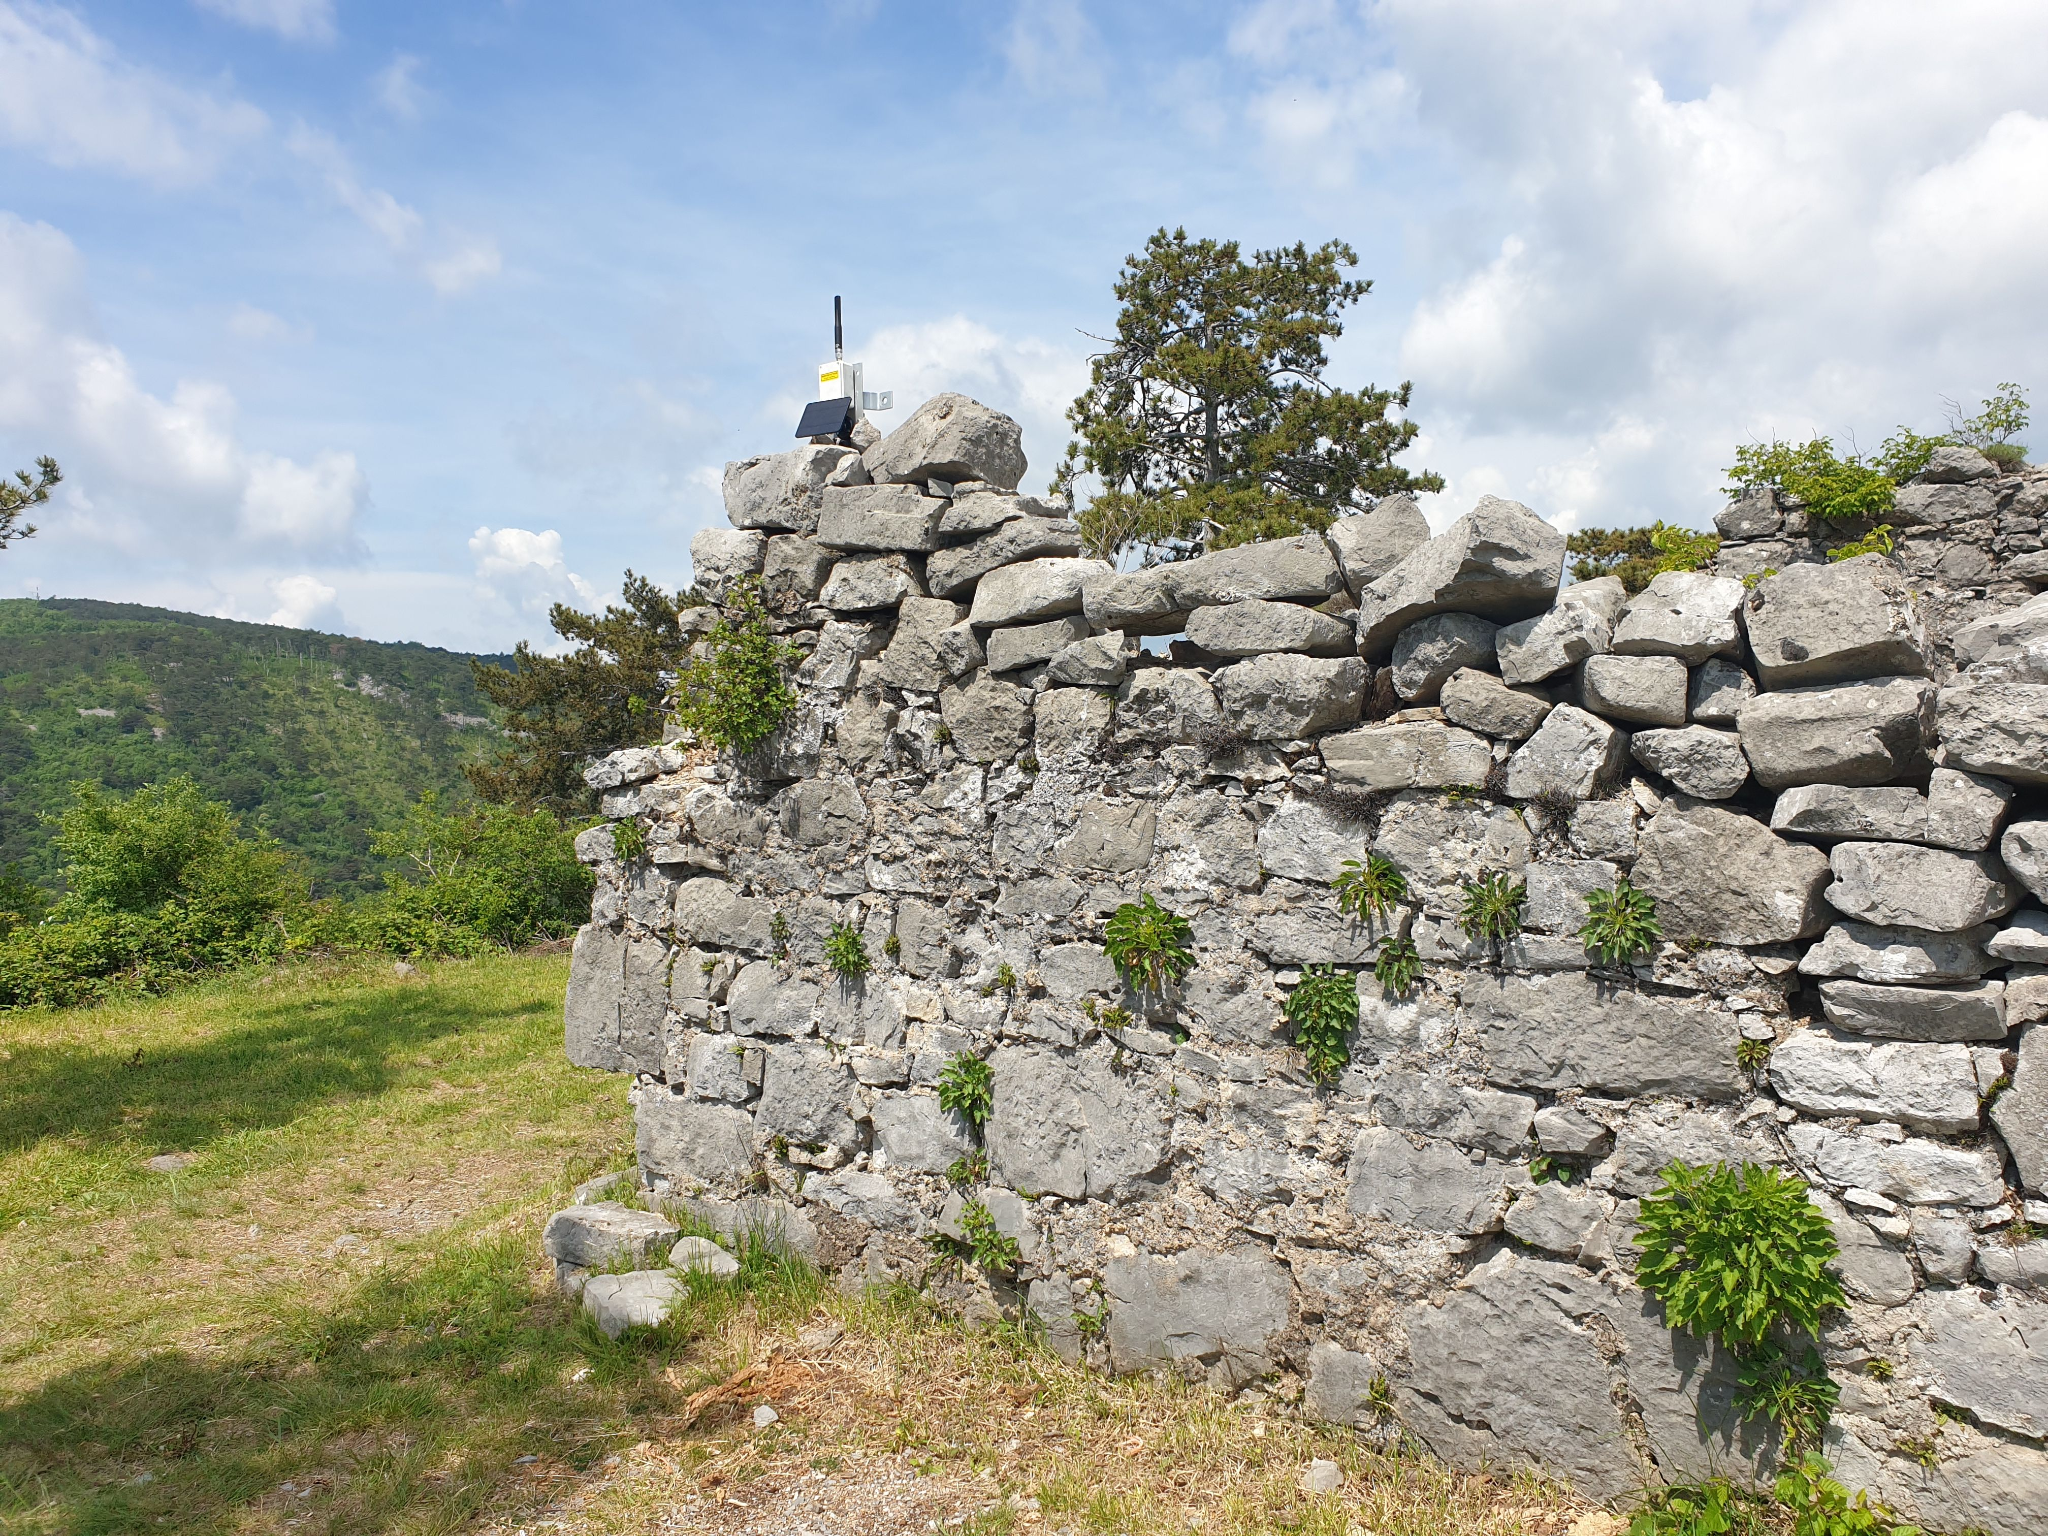
\includegraphics[width=\textwidth]{fotografije/sv-katarina-staticno-vozlisce.png}
\caption{Statično vozlišče na Sv. Katarini, !7369fb6a, 517~m nadmorske višine.}
\label{fig:sv-katarina-staticno-vozlisce}
\end{figure}

\begin{figure}[H]
\centering
\includegraphics[width=\textwidth]{fotografije/eksperimentalna-evalvacija-zemljevid-poti.jpg}
\caption{Zemljevid lokacij oddajanja in lokacij sprejemnikov}
\label{fig:eksperimentalna-evalvacija-zemljevid}
\end{figure}

Med meritvami se je vozilo, na katerem je bilo nameščeno mobilno vozlišče, premikalo po izbranem geografskem območju. Mobilno vozlišče je periodično oddajalo lokacijske pakete, pri čemer je bil časovni razmik med zaporednimi oddajami nastavljen na najmanj 15 sekund. S tem je bila zagotovljena skladnost z omejitvami radijskega spektra ter zmanjšana možnost preobremenitve omrežja. Višina oddajne antene na vozilu je bila približno 2 metra nad tlemi.

\begin{figure}[H]
\centering
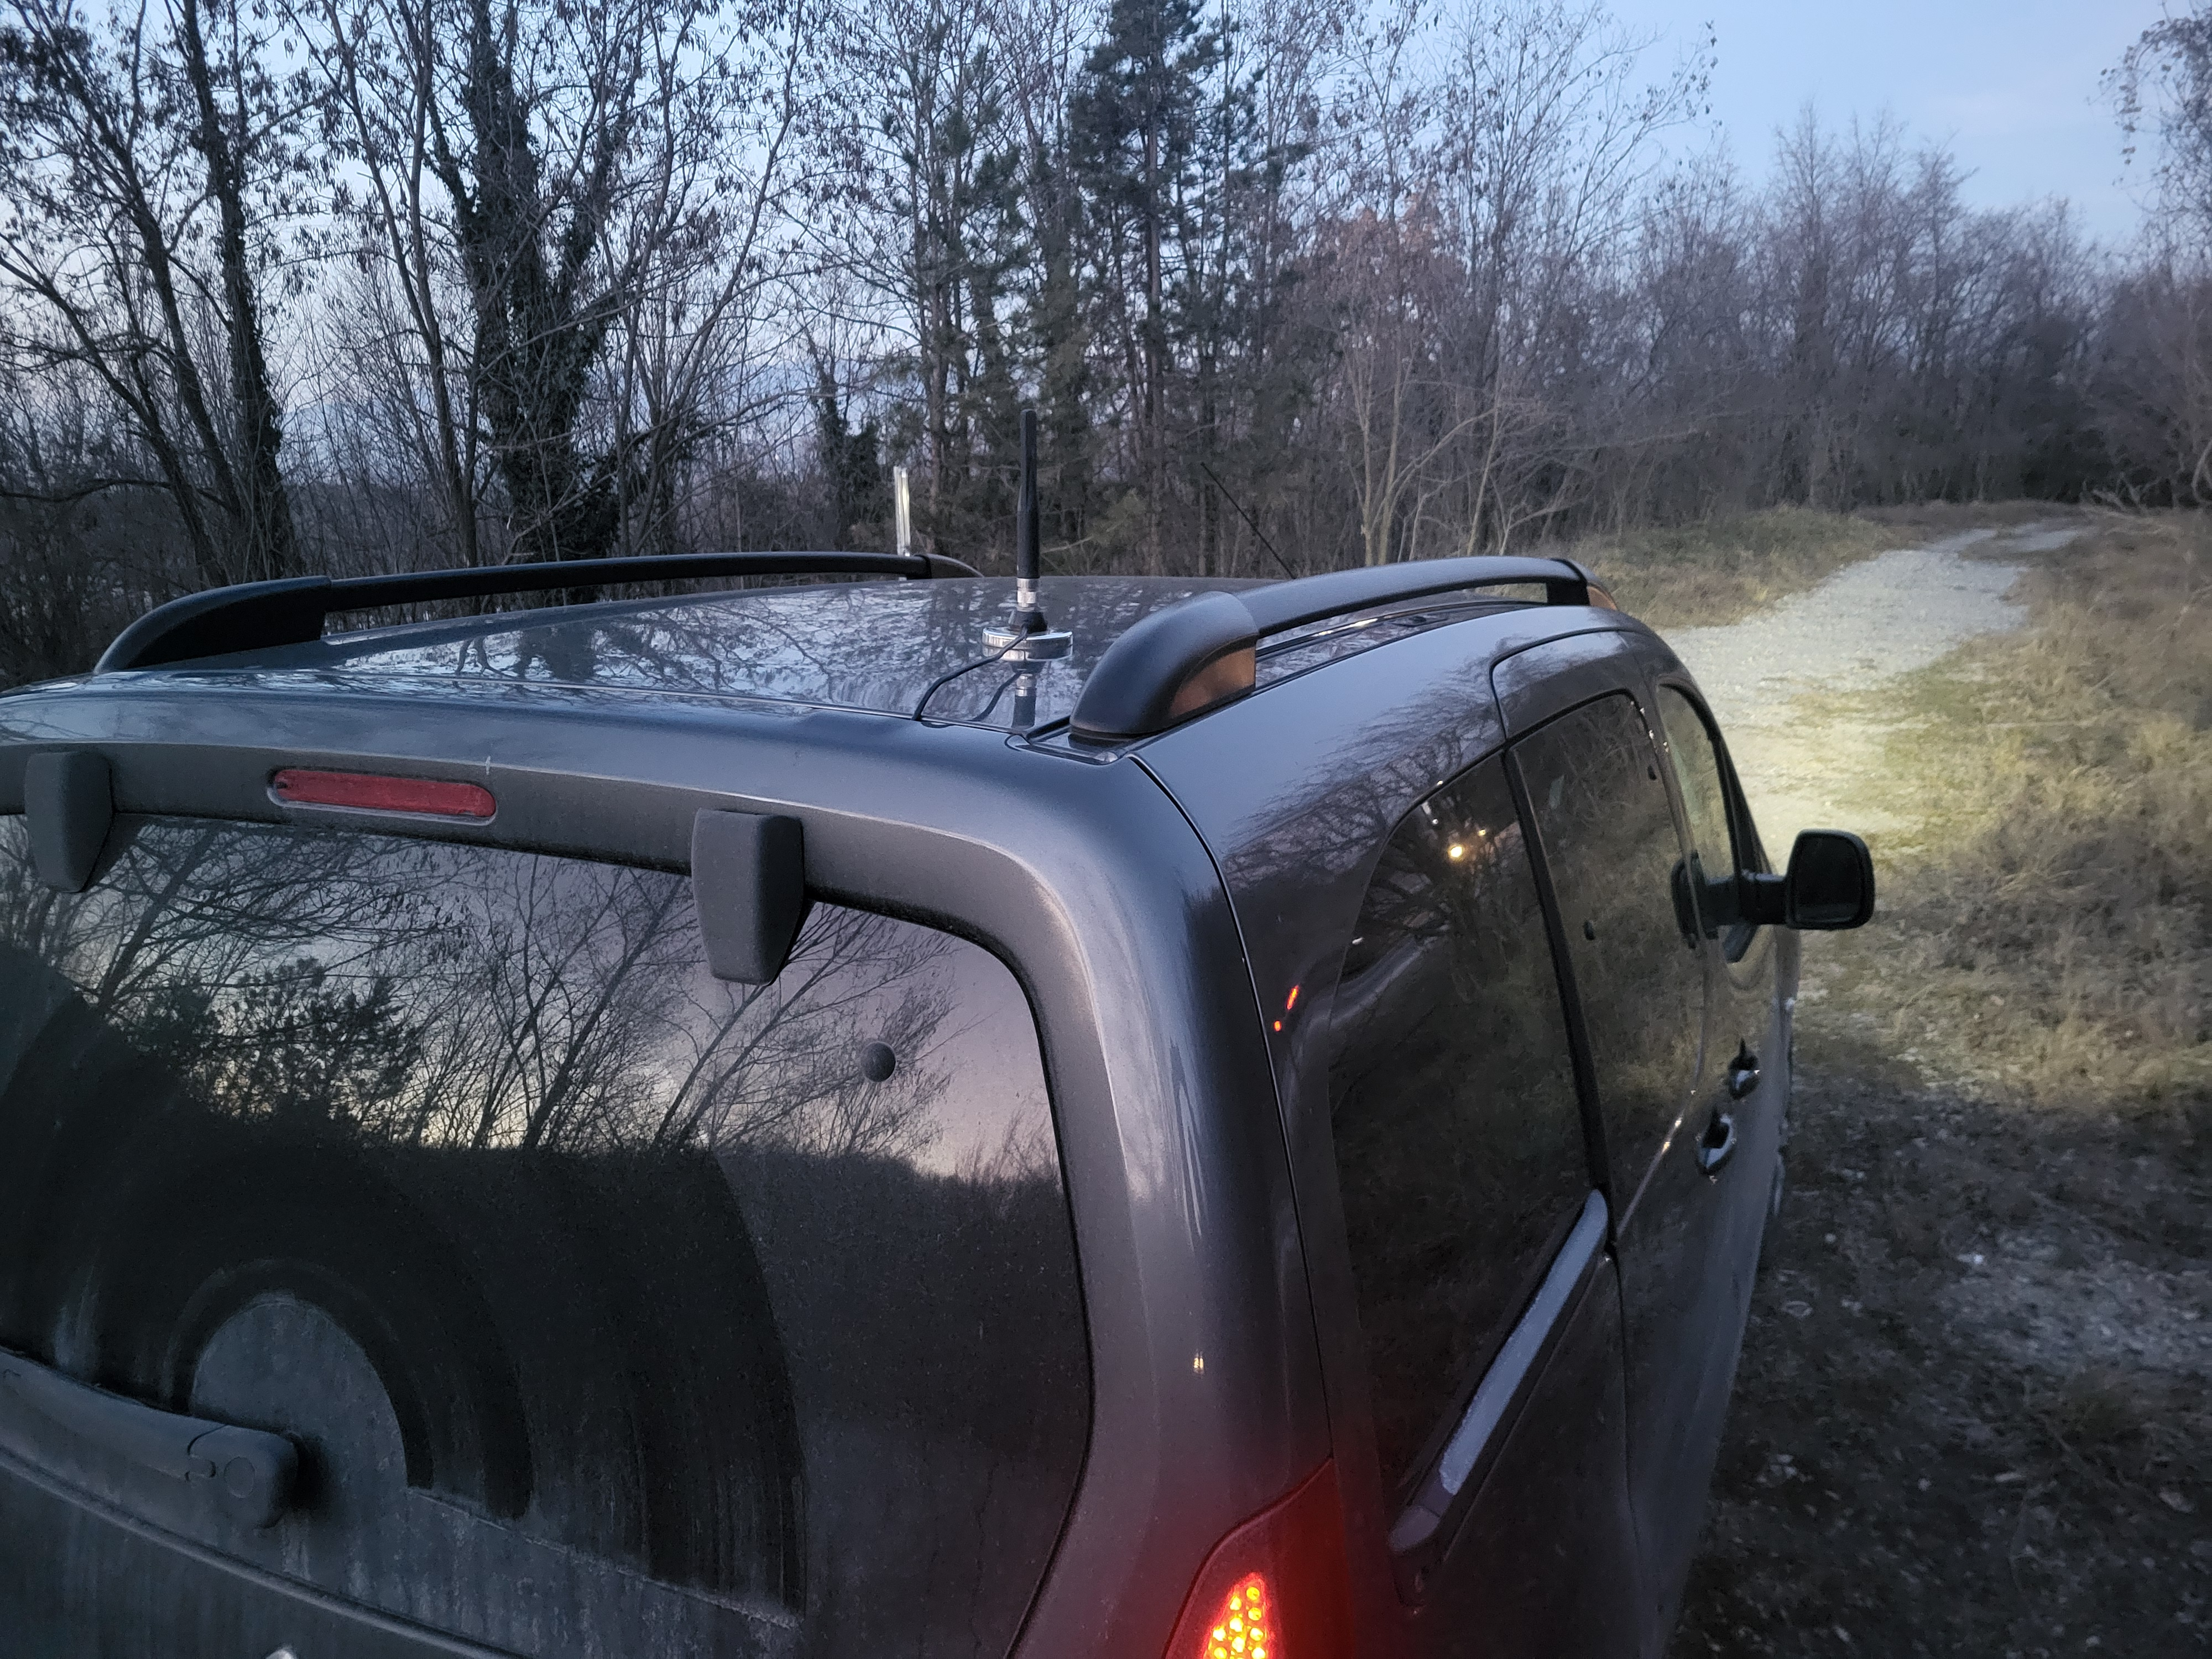
\includegraphics[width=1\textwidth]{fotografije/mobilni-node-avtomobil.jpg}
\caption{Osebni avtomobil, uporabljen kot mobilno vozlišče !42e27414.}
\label{fig:mobile-node-car}
\end{figure}

Statični vozlišči sta bili konfigurirani tako, da sta vse sprejete pakete posredovali prek protokola MQTT na osrednji strežnik. Na strežniku so se podatki samodejno shranjevali v podatkovno bazo skupaj z metapodatki, ki vključujejo čas prejema, identifikacijo oddajnika in sprejemnika ter izmerjeno jakost signala (RSSI).

Na ta način je bila vzpostavljena celovita zbirka merilnih podatkov, ki je omogočila analizo dosega, stabilnosti povezave ter prostorske porazdelitve jakosti signala. Zbrane meritve so bile v nadaljevanju uporabljene za primerjavo z rezultati simulacij in za ovrednotenje natančnosti uporabljenega radijskega modela.


\section{Rezultati}
Sprejemnik \texttt{!7369fb6a} je v času meritev skupno sprejel 434 paketov, medtem ko je nižje ležeči sprejemnik \texttt{!75f19024} sprejel 363 paketov. Razlika v številu sprejetih paketov je posledica različne višine namestitve anten in posledično drugačnih propagacijskih pogojev.

Sliki~\ref{fig:7369fb6a-val} in~\ref{fig:75f19024-val} prikazujeta primerjavo izmerjenih in simuliranih vrednosti RSSI za oba sprejemnika. Opaziti je, da simulacija v splošnem pravilno sledi trendu sprememb jakosti signala glede na položaj mobilnega vozlišča, vendar v določenih odsekih izrazito podcenjuje ali precenjuje dejansko izmerjene vrednosti.

\begin{figure}[H]
\centering
\includegraphics[width=1\textwidth]{fotografije/!7369fb6a_val.png}
\caption{Graf sprejemnika \texttt{!7369fb6a}, ki prikazuje meritev in simulacijo}
\label{fig:7369fb6a-val}
\end{figure}

\begin{figure}[H]
\centering
\includegraphics[width=1\textwidth]{fotografije/!75f19024_val.png}
\caption{Graf sprejemnika \texttt{!75f19024}, ki prikazuje meritev in simulacijo}
\label{fig:75f19024-val}
\end{figure}

Razlika med izmerjeno in simulirano jakostjo signala je bila definirana kot
\[
\Delta RSSI = RSSI_{\text{meritev}} - RSSI_{\text{simulacija}},
\]
kjer negativna vrednost pomeni, da je simulacija podcenila dejansko izmerjeno jakost signala, pozitivna vrednost pa pomeni njeno precenjevanje.

Z namenom podrobnejše analize so bili podatki razdeljeni v pet kategorij glede na geometrijske in propagacijske pogoje med oddajnikom in sprejemnikom:

\begin{itemize}
    \item \textbf{Vsi paketi} – združena napaka vseh prejetih paketov, ne glede na propagacijske pogoje.
    \item \textbf{LOS} – napake paketov v primerih, ko sta imela oddajnik in sprejemnik med seboj vidno linijo (angl. \emph{line of sight}).
    \item \textbf{NLOS} – napake paketov v primerih, ko med oddajnikom in sprejemnikom ni bilo vidne linije.
    \item \textbf{NF60} – napake paketov v primerih, ko je bila prva Fresnelova cona prekrita približno do 60~\%.
    \item \textbf{NFF} – napake paketov v primerih, ko je bila prva Fresnelova cona v celoti prekrita.
\end{itemize}

Na obeh grafih~\ref{fig:7369fb6a-diff-box} in~\ref{fig:75f19024-diff-box} lahko vidimo, da je simulacija NLOS povezave močno podcenila. Ostale vrste povezav pa se gibljejo na precenjenem območju. 

\begin{figure}[H]
\centering
\includegraphics[width=1\textwidth]{fotografije/!7369fb6a_diff.png}
\caption{Graf sprejemnika \texttt{!7369fb6a}, ki prikazuje napako med meritvijo in simulacijo, glede na vidnost.}
\label{fig:7369fb6a-diff}
\end{figure}

\begin{figure}[H]
\centering
\includegraphics[width=1\textwidth]{fotografije/!75f19024_diff.png}
\caption{Graf sprejemnika \texttt{!75f19024}, ki prikazuje napako med meritvijo in simulacijo, glede na vidnost.}
\label{fig:75f19024-diff}
\end{figure}

Porazdelitev napak po posameznih kategorijah je prikazana na slikah~\ref{fig:7369fb6a-diff-box} in~\ref{fig:75f19024-diff-box}. Škatle z brki jasno pokažejo, da je razpršenost napak močno odvisna od vidnosti in stopnje oviranosti Fresnelove cone.

\begin{figure}[H]
\centering
\includegraphics[width=1\textwidth]{fotografije/!7369fb6a_diff_box.png}
\caption{Graf sprejemnika \texttt{!7369fb6a}, ki prikazuje napako med meritvijo in simulacijo, glede na vidnost.}
\label{fig:7369fb6a-diff-box}
\end{figure}

\begin{figure}[H]
\centering
\includegraphics[width=1\textwidth]{fotografije/!75f19024_diff_box.png}
\caption{Graf sprejemnika \texttt{!75f19024}, ki prikazuje napako med meritvijo in simulacijo, glede na vidnost.}
\label{fig:75f19024-diff-box}
\end{figure}


Sliki~\ref{fig:7369fb6a-diff-vs-length} in~\ref{fig:75f19024-diff-vs-length} prikazujeta tudi odvisnost napake simulacije $\Delta RSSI$ od dolžine povezave. Vsaka točka predstavlja razliko med izmerjeno in simulirano vrednostjo RSSI pri določeni razdalji med oddajnikom in sprejemnikom.

Pri sprejemniku \texttt{!7369fb6a} je opazna izrazita negativna korelacija med dolžino povezave in napako simulacije, kar potrjuje tudi linearni regresijski model z razmeroma visokim koeficientom determinacije ($R^2 = 0.428$). To pomeni, da simulacija z naraščajočo razdaljo vse pogosteje podcenjuje dejansko izmerjeno jakost signala.

Pri sprejemniku \texttt{!75f19024} z nižjo nadmorsko višino je korelacija med razdaljo in napako bistveno šibkejša ($R^2 = 0.061$), kar kaže na večji vpliv lokalnih dejavnikov, kot so višina antene, ovire in topografija. Kljub temu je tudi v tem primeru opazen splošen trend naraščanja absolutne napake z razdaljo.

Rezultati potrjujejo, da natančnost simulacij z uporabo determinističnega propagacijskega modela upada z naraščajočo dolžino povezave, zlasti v primerih brez vidne linije, kjer imajo lokalni propagacijski pojavi bistveno večji vpliv kot sama razdalja.


\begin{figure}[H]
\centering
\includegraphics[width=\textwidth]{fotografije/!7369fb6a_diff_vs_length_non_los.png}
\caption{Odvisnost napake simulacije od dolžine povezave za sprejemnik \texttt{!7369fb6a}}
\label{fig:7369fb6a-diff-vs-length}
\end{figure}

\begin{figure}[H]
\centering
\includegraphics[width=\textwidth]{fotografije/!75f19024_diff_vs_length_non_los.png}
\caption{Odvisnost napake simulacije od dolžine povezave za sprejemnik \texttt{!75f19024}}
\label{fig:75f19024-diff-vs-length}
\end{figure}


\section{Kalibracija na podlagi meritev}

Na podlagi rezultatov eksperimentalne evalvacije je bilo ugotovljeno, da se v primerih brez vidne linije (NLOS) napaka simulacije sistematično spreminja z razdaljo med oddajnikom in sprejemnikom. Opazna je bila odvisnost med dolžino povezave in razliko med izmerjeno ter simulirano vrednostjo RSSI, kar kaže na prisotnost razdaljsko odvisnega sistematičnega odklona v uporabljenem propagacijskem modelu.

Z namenom izboljšanja natančnosti napovedi je bila izvedena kalibracija simulacijskih rezultatov na podlagi dejanskih meritev. Kalibracija je temeljila na linearni regresiji, s katero je bila modelirana odvisnost napake simulacije od razdalje. Izračunani linearni regresijski model je bil nato uporabljen za korekcijo simuliranih vrednosti RSSI.

Za preprečevanje pristranskosti in preverjanje posplošljivosti kalibracije so bili razpoložljivi podatki razdeljeni na dva disjunktna dela. Prva polovica meritev je bila uporabljena za izračun regresijskega modela, druga polovica pa za neodvisno evalvacijo učinkovitosti kalibracije. Meritve v obeh delih so bile izvedene na različnih odsekih poti, kar zagotavlja, da kalibracija ni prilagojena specifični trasi ali lokalnim značilnostim okolja.

Na sliki~\ref{fig:7369fb6a-box-before} je prikazana porazdelitev napak simulacije glede na propagacijske pogoje pred izvedeno kalibracijo, medtem ko slika~\ref{fig:7369fb6a-box-after} prikazuje porazdelitev napak po uporabi kalibracijskega modela.

\begin{figure}[H]
\centering
\includegraphics[width=\textwidth]{fotografije/!7369fb6a_diff_box_2_half.png}
\caption{Porazdelitev napake simulacije glede na propagacijske pogoje pred kalibracijo za sprejemnik \texttt{!7369fb6a}}
\label{fig:7369fb6a-box-before}
\end{figure}

\begin{figure}[H]
\centering
\includegraphics[width=\textwidth]{fotografije/!7369fb6a_diff_box_2_half_optimized.png}
\caption{Porazdelitev napake simulacije glede na propagacijske pogoje po kalibraciji za sprejemnik \texttt{!7369fb6a}}
\label{fig:7369fb6a-box-after}
\end{figure}

Učinek kalibracije je bil ocenjen s primerjavo porazdelitve napak pred in po kalibraciji. Škatle z brki (box-plot) jasno pokažejo, da se je po kalibraciji mediana napak v NLOS pogojih približala vrednosti 0~dB, kar kaže na zmanjšanje sistematičnega odklona simulacijskih rezultatov.

Rezultati potrjujejo, da lahko preprosta linearna kalibracija na podlagi terenskih meritev izboljša ujemanje med simuliranimi in izmerjenimi vrednostmi RSSI, zlasti v NLOS pogojih, kjer osnovni propagacijski model deluje konzervativno.


\section{Razprava}

Rezultati eksperimentalne evalvacije kažejo jasno odvisnost natančnosti simulacij od propagacijskih pogojev. V primerih z vidno linijo (LOS) je razlika med izmerjenimi in simuliranimi vrednostmi RSSI relativno majhna, mediane napak pa se pri obeh sprejemnikih gibljejo okoli 10~dB. Takšna stopnja ujemanja potrjuje, da uporabljeni radijski model v pogojih vidne linije ustrezno opisuje osnovne propagacijske mehanizme, kar je skladno z ugotovitvami iz literature~\cite{6618611}.

V primerih brez vidne linije (NLOS) so odstopanja bistveno večja, pri čemer se mediane napak gibljejo okoli 20~dB. Simulacija v teh pogojih pogosto podcenjuje dejanski doseg povezave, kar se odraža v negativni sistematični napaki in izrazito večji razpršenosti podatkov. Posamezna odstopanja presegajo 40~dB, kar kaže na omejitve determinističnega propagacijskega modela pri opisovanju kompleksnih mehanizmov širjenja signala v razgibanem terenu.

Dodatna analiza je pokazala, da ima dolžina povezave vpliv na napako simulacije, zlasti v pogojih brez vidne linije. Z naraščajočo razdaljo med oddajnikom in sprejemnikom se sistematično povečuje absolutna napaka med izmerjenimi in simuliranimi vrednostmi RSSI, kar potrjuje negativna korelacija, ugotovljena z linearno regresijsko analizo.

\chapter{Diskusija}

\section{Izboljšave}
Med razvojem aplikacije se je bilo treba osredotočiti predvsem na implementacijo ključnih funkcionalnosti, ki so bile nujne za doseganje ciljev diplomske naloge. Zaradi časovnih omejitev in kompleksnosti posameznih problemov vseh načrtovanih idej ni bilo mogoče v celoti realizirati. Nekatere izboljšave bi zahtevale bistveno več razvojnega časa, druge pa uporabo dodatnih tehnologij ali podatkovnih virov, ki presegajo obseg te naloge. V nadaljevanju so zato predstavljene izbrane nadgradnje, ki bi lahko v prihodnje dodatno izboljšale zmogljivost, uporabnost in razširljivost aplikacije.

\subsection{Naprednejše simulacijsko orodje}
Ena izmed pomembnih možnih izboljšav sistema bi bila zamenjava simulacijskega orodja SPLAT! z naprednejšo rešitvijo za modeliranje širjenja radijskega signala. Čeprav SPLAT! omogoča relativno natančne izračune na podlagi topografije in Fresnelovih con, ima več omejitev, ki otežujejo njegovo uporabo v sodobnih aplikacijah.

SPLAT! ne podpira uporabe različnih tipov talne in prostorske oviranosti (clutter), kot so gozdovi, urbana območja ali stavbe, temveč uporablja enoten parameter za višino ovir. Prav tako je orodje zasnovano kot enonitna (single-threaded) aplikacija, kar bistveno podaljša čas izvajanja zahtevnejših simulacij. Dodatna omejitev je podpora izključno za SRTM digitalne modele višin, brez možnosti enostavne uporabe drugih virov ali višjih ločljivosti.

Z vidika integracije predstavlja SPLAT! izziv, saj je primarno namenjen uporabi prek ukazne vrstice, ponuja omejen nabor izhodnih formatov ter ni zasnovan kot knjižnica ali storitev. To zahteva obsežno obdelavo vmesnih datotek in otežuje neposredno povezovanje z aplikacijami, kakršna je razvita rešitev v tej nalogi.

Uporaba sodobnejšega simulacijskega orodja, ki bi podpiralo večnitno izvajanje, napredne modele oviranosti, širši nabor vhodnih in izhodnih podatkov ter boljšo integracijo prek API-jev, bi lahko bistveno izboljšala zmogljivost, razširljivost in uporabno vrednost aplikacije.

\subsection{Tridimenzionalni prikaz}
Uvedba tridimenzionalnega (3D) prikaza bi uporabniku omogočila boljšo prostorsko predstavo o razgibanosti terena in njegovem vplivu na širjenje radijskega signala. V primerjavi z obstoječim 2D prikazom bi 3D vizualizacija jasneje izpostavila višinske razlike, grebene in doline, ki pogosto predstavljajo ključne ovire pri vzpostavljanju povezav.

Takšen prikaz bi olajšal prepoznavanje ovir na poti signala ter omogočil preglednejšo vizualizacijo poteka vidne linije in Fresnelovih con. Uporabnik bi tako hitreje razumel, kje pride do zakritja in kako spremembe višine ali lokacije anten vplivajo na kakovost povezave.

\begin{figure}[htb]
\centering
\includegraphics[width=1\textwidth]{fotografije/izboljsave_3d_prikaz.png}
\caption{Posnetek zaslona 3D modela reliefa}
\label{fig:izboljsave-3d-prikaz}
\end{figure}

\subsection{Orodna vrstica za prostorsko analizo}
Ena izmed možnih izboljšav uporabniškega vmesnika bi bila uvedba dodatne orodne vrstice na zemljevidu, ki bi omogočala osnovna orodja za prostorsko analizo. Uporabnik bi lahko na zemljevidu risal preproste geometrijske oblike, kot so točke, linije in poligoni, z namenom boljše prostorske predstave in označevanja interesnih območij.

Orodna vrstica bi vključevala tudi preprosto orodje za hitro preverjanje vidne linije (LOS) med izbranima točkama, ki bi služilo kot orientacijska pomoč pred zagonom podrobnejših simulacij. Poleg tega bi bila na voljo funkcionalnost »pipete«, ki bi omogočala neposredno zajemanje in kopiranje geografskih koordinat iz zemljevida, kar bi olajšalo natančen vnos lokacij in izmenjavo podatkov z drugimi sistemi.

\subsection{Izvoz rezultatov v standardne GIS formate}
Ena izmed pomembnih nadgradenj aplikacije bi bila razširitev možnosti izvoza rezultatov simulacij in analiz v standardne geografske podatkovne formate. Podpora formatom, kot so SHP, KML, GeoJSON in PDF, bi uporabniku omogočila nadaljnjo obdelavo podatkov v zunanjih GIS orodjih ali enostavno predstavitev rezultatov.

Izvoz v vektorske in rastrske formate bi omogočil uporabo rezultatov v profesionalnih okoljih, kot so QGIS ali ArcGIS, ter lažjo izmenjavo podatkov z drugimi deležniki. PDF izvoz pa bi bil primeren za poročila, dokumentacijo in predstavitve, kjer interaktivnost ni potrebna, pomembna pa je jasna vizualna predstavitev rezultatov.

\subsection{Vnos in primerjava terenskih meritev}
Dodatna nadgradnja aplikacije bi bila možnost vnosa dejanskih terenskih meritev, s katerimi bi bilo mogoče preverjati točnost simulacijskih rezultatov. Uporabnik bi lahko v aplikacijo uvozil izmerjene vrednosti, kot je RSSI, skupaj z geografskimi koordinatami merilnih točk.

Sistem bi omogočal vizualno in numerično primerjavo med izmerjenimi podatki in rezultati simulacij, na primer z izrisom meritev na zemljevidu ali z izračunom odstopanj. Na ta način bi bilo mogoče hitro prepoznati območja, kjer model odstopa od realnih razmer, ter oceniti zanesljivost simulacij v različnih okoljih.

\chapter{Zaključek}

V diplomski nalogi je bila obravnavana problematika načrtovanja LoRa omrežij. Pregled obstoječih orodij je pokazal, da večina rešitev bodisi ponuja omejeno funkcionalnost bodisi ni prilagojena sodobnim potrebam uporabnikov, ki želijo celovit, razširljiv in odprtokoden sistem za podporo odločanju pri postavitvi omrežij.

Glavni rezultat naloge je razvoj odprtokodne spletne aplikacije \emph{RF Site Planner}. Aplikacija temelji na propagacijskem orodju SPLAT! ter predstavlja
nadgradnjo obstoječe odprtokodne rešitve Meshtastic Site Planner~\cite{meshtasticSitePlanner}.
Izvorno funkcionalnost simulacije pokritosti smo razširili z dodatnimi
možnostmi, kot so analiza vidne linije, iskanje optimalnih lokacij
oddajnikov ter izboljšana obdelava in vizualizacija prostorskih podatkov.

Eksperimentalna evalvacija na podlagi dejanskih terenskih meritev je pokazala, da simulacije v pogojih vidne linije dosegajo zadovoljivo stopnjo ujemanja z izmerjenimi vrednostmi. V pogojih brez vidne linije so bila odstopanja večja, kar je skladno z znanimi omejitvami determinističnih propagacijskih modelov. Kljub temu rezultati potrjujejo, da je razvito orodje uporabno za praktično načrtovanje LoRa omrežij, zlasti v fazi izbire lokacij oddajnikov in grobe ocene pokritosti. Dodatno je bila prikazana možnost izboljšanja natančnosti simulacij s preprosto kalibracijo na podlagi meritev, kar odpira prostor za nadaljnje nadgradnje.

Prispevek naloge ni zgolj v funkcionalni aplikaciji, temveč tudi v odprti zasnovi rešitve. Celotna izvorna koda aplikacije je javno dostopna in objavljena v repozitoriju GitHub:

\begin{center}
\url{https://github.com/KomelT/rf-site-planner}
\end{center}

S tem je omogočeno, da razvito orodje služi kot osnova za nadaljnji razvoj, prilagoditve specifičnim scenarijem uporabe ter vključevanje naprednejših propagacijskih modelov ali dodatnih podatkovnih virov. Naloga tako predstavlja praktičen prispevek k odprtokodni skupnosti in hkrati uporabno orodje za vse, ki se ukvarjajo z načrtovanjem in analizo LoRa ali drugih brezžičnih omrežij v realnem prostoru.


%\cleardoublepage
%\addcontentsline{toc}{chapter}{Literatura}

% če imaš težave poravnati desni rob bibliografije, potem odkomentiraj spodnjo vrstico
\raggedright

%\printbibliography[heading=bibintoc,type=article,title={Članki v revijah}]

%\printbibliography[heading=bibintoc,type=inproceedings,title={Članki v zbornikih}]

%\printbibliography[heading=bibintoc,type=incollection,title={Poglavja v knjigah}]

% v zadnji verziji diplomskega dela običajno združiš vse tri vrste referenc v en sam seznam in
% izpustiš delne sezname
\printbibliography[heading=bibintoc,title={Literatura}]

\end{document}
